\chapter{\acl{sota}}
\label{chapter:sota}
On this chapter we detail the foundation for this work, by conducting a thoroughly and extensive analysis to the current state of the art of several topics required on our work, giving some considerations about which approaches are followed and why.

This chapter is organized as follows. Section~\ref{sec:sota:software-middleware} contains a brief analysis of the current possibilities for middleware and message passing software between programs and systems, allowing a better code workflow and modularity. On Section~\ref{sec:sota:datasets}, an analysis of the currently available online datasets for autonomous driving is given, along with a comparison of their key features. Section~\ref{sec:sota:camera} details the usage of camera in computer vision applications, its geometry, intrinsic calibration and image processing libraries. On Section~\ref{sec:sota:lidar}, considerations on automotive \ac{lidar} are given regarding its construction and technology, accompanied by an analysis of point cloud manipulation software. Having the camera and \ac{lidar} detailed, an in-depth analysis of their extrinsic calibration procedures is given. Section~\ref{sec:sota:sensor-fusion} details three different techniques of sensor-fusion between camera and \ac{lidar}. On Section~\ref{sec:sota:object-detection}, object detection on image is detailed, presenting some techniques and commonly used  public image datasets for training. Lastly, Section~\ref{sec:sota:lidar-interference} gathers and compares all the work on \ac{lidar} interference, either from the standpoint of an attacker wanting to purposely interfere with a \ac{lidar} and academic research seeking to understand the phenomena.


\section{Middleware Software and Message Passing}
\label{sec:sota:software-middleware}
Analyzing the \ac{lidar} interference is our primary goal, but several other objectives have been established for this work, on Section~\ref{sec:introduction:objectives}. Fulfilling them requires using a \ac{lidar} and a camera, through a multi-sensor approach, which enables us to analyze interference as a pure interference phenomenon between sensors and understanding its impact on \ac{roi}.

Developing such software, however, requires more than standalone program files, due to the complex interactions between sensors and data. Is crucial, for the success of this work, that standalone programs, which perform their own set of tasks, could communicate it each other, seamlessly, exchanging data and commands.

With those considerations, we require the usage of a middleware, a software layer that can communicate directly with the operative system kernel and hardware devices, abstracting its behavior through an \ac{api} that allows for the programs to communicate with the hardware devices, the kernel and amongst themselves\cite{Etzkorn2017, Huang2010}. Such software also implements a message passing infrastructure between peer-to-peer and/or client-server communication, for data exchange and marshalling~\cite{Etzkorn2017}.

\subsection{Middleware software libraries and Robotics} 
Several middleware libraries, written in many languages, are available online, capable of message passing between programs:

\begin{itemize}
	\item \textbf{PocoLibs:} an Open-Source library developed by OpenRobots that allows for communication between process on a computer system, with support for real-time~\cite{Pocolibs};
	\item \textbf{\ac{lcm} library:} focused on low latency and high-bandwidth, this library is developed with real-time systems in mind, providing data marshalling and message passing between a publisher and subscriber~\cite{Huang2010b};
	\item \textbf{ZeroMQ:} a framework with bindings for many languages that can be used to transport messages between process, \ac{tcp} or multicast, for example. Allows a series of different connection types~\cite{ZeroMQ}.
	\item \textbf{\ac{yarp}:} a collection of programs, written in C++, focused on enabling peer-to-peer communication, supporting \ac{tcp}, \ac{udp}, multicast, amongst many other protocols~\cite{Metta2006};
	\item \textbf{\ac{ros}:} a complex and extensive framework for developing and test robot software. It was developed with the goal of simplifying the task of building complex and robust robot behavior, independently of the hardware and mechanical platform. Offers a collection of tools, libraries and conventions~\cite{ROS};
	\item \textbf{\ac{ros} 2:} a more recent iteration of the \ac{ros} development, focused on extending \ac{ros} capabilities to new use cases, such as multiple robot teams, small embedded platforms and real-time systems~\cite{ROS2};
	\item \textbf{\ac{mrpt}:} a mobile robot library, written in C++, which aims to provide a set of tools and libraries for computer vision, motion planning and \ac{slam}. It also directly supports hardware and implements message passing middleware~\cite{MRPT};
\end{itemize}

While the first 4 listed alternatives are focused on generic communication between processes\footnote{Despite its name, \acf{yarp} is not a robotic operative system or framework, but instead a message passing framework for robots.}, inter-process and common know communication protocols, the last 3 are oriented for robotics, providing a comprehensive set of tools for robotics development besides the message passing. The latter is preferred, since it has the potential to unburden us from the development of generic debug tools, data visualization and logging. Therefore, we exclude PocoLibs~\cite{Pocolibs}, \ac{lcm} library~\cite{Huang2010b}, ZeroMQ~\cite{ZeroMQ} and \ac{yarp}~\cite{Metta2006}.

Since our work is also not oriented for real-time applications, we will not use \ac{ros} 2~\cite{ROS2}. Comparing the three robotic platforms, \ac{mrpt} is focused on robot mobility, \ac{slam}, computer vision and motion planning, while \ac{ros} is more generic and widely used, containing all the capabilities of \ac{mrpt}. Also, \ac{ros} is more widely accepted and has a larger community.

Therefore, for the middleware layer and message passing we will use \ac{ros}, taking also advantage of all the other tools it provides and its Open-Source third-party libraries.

\subsection{\ac{ros} version}
\ac{ros} has two long term support versions, whose release schedule is synchronized with Ubuntu operative system~\cite{ROS}. At the time of writing, two versions are currently available: \textit{\ac{ros} Kinetic Kame} and \textit{\ac{ros} Melodic Morenia}.

\textit{\ac{ros} Kinetic} was released in May 2016 and support ends on April 2021. \textit{\ac{ros} Melodic} was released in May 2018 and its end of life is on May 2023. At the time of this work, the most recent version, \textit{\ac{ros} Melodic}, is stable, free of release bugs and most of the \textit{\ac{ros} Kinetic} libraries have already been ported. Therefore, our choice relies on \textit{\ac{ros} Melodic Morenia}, since more concretely, version \texttt{1.14.3}. To work with this version of \ac{ros}, the C++ standard used is version 14.


\section{Datasets}
\label{sec:sota:datasets}

Training an autonomous vehicle to be capable of driving itself is a complex challenge with multiple parts and problems to solve: recognizing other road users (people, vehicles, cyclists); understanding traffic signs; track and estimate the movement of the road users; plan the path; accurate modelling of the environment; amongst many others. Developing models that can describe and solve these problems, but also testing systems and other software, requires huge amounts of data.
%To both train neural networks and other genetic algorithms,

To accelerate this progress, a collaborative effort is being made to release free datasets online for public usage under permissive licenses. These datasets vary in their objective, sensory data available, conditions which data has been acquired, driving conditions and format on which they are provided, amongst other aspects. 

Despite this work not intending to study autonomous driving, the algorithms developed for calibration, sensor fusion and computing the correspondence between objects of interest in image and point cloud are not exclusive for application on datasets with interference. Therefore, using public available datasets (which no not have interference) not only allows the development of those algorithms before experimental data can be gathered, but also widen the applicability of such work, without losing their applicability to the particular situation of \ac{lidar} interference.

During the months when this research work was carried, several new datasets were made available online, such as nuScenes~\cite{nuScenes2019} and Waymo~\cite{Waymo}. Since no new contributions to this work were expected from their usage, no further research on these was carried. 

Other older datasets were considered and tested. On the next sections, a brief summary is given about the ones that have sensory data from camera and \ac{lidar}. Those were the candidates to be used on this work.

\subsection{Ford Campus \acl{lidar} dataset}
Gathered in 2009, in Michigan, the Ford Campus \ac{lidar} dataset contains camera, \ac{lidar}, \acf{imu} and \acf{gps} data\cite{Pandey2011}. The dataset consists of two test scenarios, one inside the Ford Research campus and the other on downtown Dearborn. A small subset of the former test scenario is also provided.

The modified Ford F-250 pickup truck, which can be seen on figure~\ref{fig:sota:ford_sensors}, uses 3 sensors for navigation~\cite{Pandey2011}: one 3D \ac{lidar}, Velodyne HDL-64E \ac{lidar}~\cite{VelodyneHDL64}; one camera: Point Grey Ladybug3 omnidirectional camera; and two 2D \acp{lidar}: Riegl LMS-Q120 lidar. For more details about the sensors, their relative positioning, data formats and files see~\cite{Pandey2011}.

\begin{figure}[!ht]
	\centering
	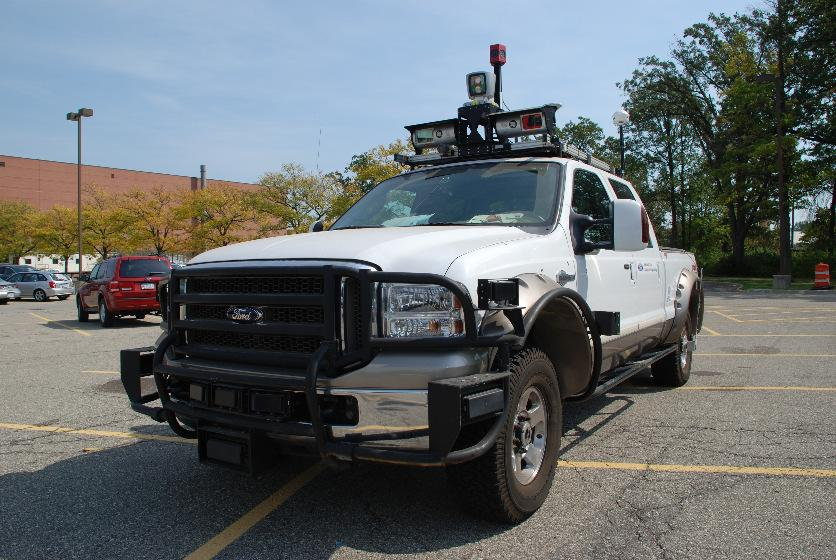
\includegraphics[width=0.5\textwidth]{img/sensor_fusion/ford_sensors.jpg}
	\caption{Ford 250 pickup equipped with some of the sensors described in the section~\ref{sec:introduction:scope_motivation}. On the top, the Ladybug omnidirectional camera, on the back the \ac{imu} and \ac{gps} unit.}
	\label{fig:sota:ford_sensors}
\end{figure}

The data is provided in raw format, accompanied by log files with timestamps, \ac{gps} and \ac{lcm}\footnote{For more information on \acf{lcm} protocol for estimating delays between sensory data registration on master-slave systems, see~\cite{LCM}.} logs with all raw data. The images from an omnidirectional camera%, a Point Grey Ladybug3, 
are stored on \ac{ppm} and \ac{lidar} data %from a Velodyne HDL-64E
on \ac{pcap} format, from the \ac{tcp} connection socket.%; two Riegl LMS-Q120 \acp{lidar} also provide more information on the scan.

Rectified and synced data is stored in \ac{matlab} \textit{.mat} files. Along with the raw data and synced and rectified \textit{.mat} files, source code is also provided for parsing the raw data, visualizing the \ac{lcm} logs and pre-processed data on \ac{matlab}. A C and \ac{opengl} software that can render textured point clouds is also available.


\subsection{\acl{kitti} Dataset}
A well known dataset for researchers of computer vision, autonomous driving and \ac{ml}, \ac{kitti} was recorded in 2011 and released to the public in 2013. This dataset contains various driving scenarios: suburban, highways, residential and campus areas; with trucks, cars, cyclists and persons. Alongside with data for testing, calibration measures are provided for all sensors.

The test car, a Volkswagen Passat is equipped with two stereo pairs, one with color and one with gray cameras, a \ac{lidar}, an \ac{imu} and a \ac{gps} sensor, is shown on figure~\ref{fig:sota:kitti_sensors}. Data from all four cameras is stored on \ac{png} format, \ac{lidar} measurements stored as a binary float matrix, \ac{gps} and \ac{imu} are saved textually. Additionally, the raw data logs containing the timestamps and the transformations between the sensors are also provided. Labeled data is also available for some test scenarios in \ac{xml} files.

\begin{figure}[!ht]
	\centering
	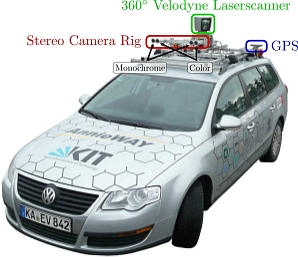
\includegraphics[width=0.5\textwidth]{img/sensor_fusion/passat_sensors.jpg}
	\caption{Volkswagen Passat equipped with the sensors described in sub-Section~\ref{subsec:introduction:scope_motivation} graphs, for the \ac{kitti} dataset. On the top, the Velodyne \ac{lidar} and below the 2 stereo pairs (color and grey). On the back, the \ac{imu} and \ac{gps} systems are present.}
	\label{fig:sota:kitti_sensors}
\end{figure}


Along with the data and calibration parameters, several tools written in C++ or \ac{matlab} are also provided. The dataset offers two types of data categories: (1) unsynced and unrectified data or (2) synced and rectified data. The latter type is the one relevant for sensory calibration purposes.

The sensory apparatus contains 2 PointGray Flea2 greyscale and color cameras, a Velodyne HDL-64E \ac{lidar}~\cite{VelodyneHDL64}, among others less relevant sensors~\cite{Geiger2013a}.

\subsection{Udacity Self-Driving Car Nanodegree Dataset}
The data from Udacity online course on self-driving car is also publicly available~\cite{udacity}. This dataset dates to 2016 and was gathered to develop level 4 autonomy vehicles, containing much more data diversity than the previous two. The data available contains images from 3 color cameras,  \ac{lidar}, \ac{imu} and \ac{gps}, among other sensory data, such as speed, braking, etc.

This information is not available in raw format, only structured in \ac{ros} \textit{.bag} files. Some tools for visualizing and interacting with their data are provided for \ac{ros}~\cite{udacity}. 

Not much information about the sensors and their positioning is publicly available, and the dataset does not contain information for calibration.

\subsection{Summary}
Table~\ref{tab:sota:datasets_comparison} summarizes all the relevant data from the datasets~\cite{udacity, Pandey2011, Geiger2013a}. While there are few differences between the relevant types of data gathered, major differences can be observed on the format in which they are provided. 

The diversity of scenarios and size of the dataset is also an aspect to consider. On this matter, \ac{kitti} and Udacity's are superior to Ford dataset, with \ac{kitti} providing the largest dataset in quantity, with already rectified and synced data. 
	
\begin{table}[H]
	 \rowcolors{4}{gray!10}{white}
	 \renewcommand{\arraystretch}{1.2}
	 \centering
	\begin{tabular}{llccc}
																& & \multicolumn{3}{c}{Datasets} \\ \cline{3-5}
																& & Ford Campus  & \acs{kitti} & Udacity \\ \midrule
																%
																& \ac{lidar}	   & \checkmark  & \checkmark & \checkmark \\ 
																& Color Camera	 & \checkmark  & \checkmark & \checkmark  \\
																& Grey Cameras   &             & \checkmark &  \\
																& Stereo Camera  &             & \checkmark & \checkmark  \\
																& Omnidirectional Camera &  \checkmark  &  &  \\
																& \acs{imu}      & \checkmark  & \checkmark & \checkmark  \\
																& \acs{gps}      & \checkmark  & \checkmark & \checkmark  \\
		\rowcolor{white}\multirow{-8}{*}{Sensors and Data} & Driving data\footnotemark & & & \checkmark \\ \hline
		\multirow{5}{*}{Data Formats and Tools} & Raw data available & \checkmark & \checkmark &  \\
																			 & Data parsing tools & \checkmark & \checkmark & \checkmark  \\
																			 & Rectified data & \checkmark & \checkmark & \checkmark \\
																			 & Synced data & \checkmark & \checkmark &  \checkmark  \\ 
																			 & Calibration parameters & \checkmark  & \checkmark  & \checkmark  \\\hline 
		\multicolumn{2}{l}{Raw data for sensors calibration} & \checkmark & \checkmark & \\
		\multicolumn{2}{l}{\ac{ros} data compatibility} &  & \checkmark\footnotemark & \checkmark \\
		\multicolumn{2}{l}{Date of acquisition} & 2009  & 2011 & 2016 \\
		\bottomrule
	\end{tabular}
\caption{Comparison between the datasets more appropriated to this thesis objectives.}
\label{tab:sota:datasets_comparison}
\end{table}
\footnotetext{Other driving data includes, but it is not limited to: vehicle speed, joints states, twist, brakes, suspension, fuel level, \ac{can} bus data, steering, tire pressure, among many others.}

\footnotetext{While Udacity dataset is the newest and provides direct out-off-the-shelf integration with \ac{ros}, that type of integration can also be achieved for \ac{kitti} by using other tools, such as \textit{kitti2bag}~\cite{TomasKrejci}.}

Comparing the 3 datasets using the information on table~\ref{tab:sota:datasets_comparison} and the previous sections, Udacity and \ac{kitti} are better suited to the purposes of this work. They provide a larger dataset than Ford, have \ac{ros} compatibility and the tools provided are open-source and not developed to be used on proprietary software.

Since Udacity dataset integrates more easily with \ac{ros} than \ac{kitti}, providing also some tools for \ac{ros} preliminary tests, learning and earlier development stages were based on this dataset. Later, due to the lack of calibration parameters and raw data for sensors calibration\footnote{Note that, despite Udacity dataset not providing data to ease the calibration of its sensors, such as camera intrinsic calibration or the extrinsic calibration between \ac{lidar} and camera, such calibration parameters can be obtained from this data. Those parameters are not as accurate as those obtained using a proper calibration setup and are out the scope of this work (being another research topic on itself) and therefore no effort will be dedicated to this topic.}, \ac{kitti} dataset was used instead.


%%%%%%%%%%%%%%%%%%%%%%%%%%%%%%%%%%%%%%%%%% CAMERA %%%%%%%%%%%%%%%%%%%%%%%%%%%%%%%%%%%%%%%%%%

\section{Camera as a sensor on \acl{cv} applications}
\label{sec:sota:camera}
Vision is the human sense most relevant to how we perceive the world and how we navigate it~\cite{Ekstrom2015, Beck1983}. Replicating this ability on machines, through the usage of cameras, is a widely researched topic on computer vision and instrumentation~\cite{Beck1983}. The most common cameras, as our eyes, take advantage of the pinhole effect: a small hole (or pin), that is used to spatially filter the non-focused light beams through an aperture or lens~\cite{Beck1983, camera_models, Sturm2010}, producing a mirrored, but focused image.

On the following sub sections, basic notions of the current status of camera models and camera calibration are given. Since this research is focused strictly to the application of a camera as a sensor on computer vision, the overview provided abstains from describing extensive research on camera technologies and camera models for the field of computer vision. From a purely working principle and technologies, several camera types can be named, such as catadioptric, plenoptic, biprism, among others~\cite{Sturm2010}. Considering consumer market, denominations such as Compact Cameras, \ac{dslr} cameras, Mirrorless (or \ac{evil} cameras) can also be used~\cite{comercial_cameras}. For further research, the reader might be interested on~\cite{comercial_cameras, Sturm2010, camera_models, Merklinger1993, Photopillers}.


\subsection{Camera Geometry}
\label{subsec:sota:camera-geometry}
A world point in a 3-dimensional Euclidean space can be represented by a vector with 3 real coordinates: $(X, Y, Z)$ and an image pixel of a digital image is typically represented as an element of a 2D matrix with integer coordinates $(u, v)$~\cite{mvg_book}. From a mathematical standpoint, a camera can be considered as a mapping tool between the world objects in three dimensions into a 2D image plan, such as depicted by equation~\eqref{eq:camera_transform}, which leads to different mathematical models used to describe the camera~\cite{mvg_book, Sturm2010}.

\begin{equation}
	\label{eq:camera_transform}
	(X, Y, Z) \xrightarrow[]{\text{transformation}} (u, v)
\end{equation}

When describing camera models, several considerations should be made~\cite{Sturm2010}:
\begin{itemize}
	\item \textbf{Central Camera Models vs Non-Central Camera Models}: quantifies the number of optical centers on a camera. A central camera has only one optical center through which all light rays pass through to reach the film and a non-central has two or more optical centers;
	\item \textbf{Global vs Local models:} indicates if the parameters of the model are the same for all the image/\ac{fov} of the camera or if different regions of the image have different parameters, respectively;
\end{itemize}

For the application currently envisioned, global central camera models are considered. For a more detailed explanation of the topics above or an extensive overview of non-classical camera models, different types of projections and other aspects of modelling cameras, see~\cite{Sturm2010, camera_models}.

\subsubsection{Pinhole Camera Model}
Based on the pinhole effect, represented on figure~\ref{fig:pinhole_effect}, the pinhole camera model is the most common camera model~\cite{camera_models}. The pinhole effect consists on using a small hole (or aperture) to spatially filter the light rays by angle of incidence, reducing the amount of light rays overlapping when coming from different incident angles through the pinhole, which otherwise would ``blur'' the image. 

\begin{figure}[H]
	\centering
	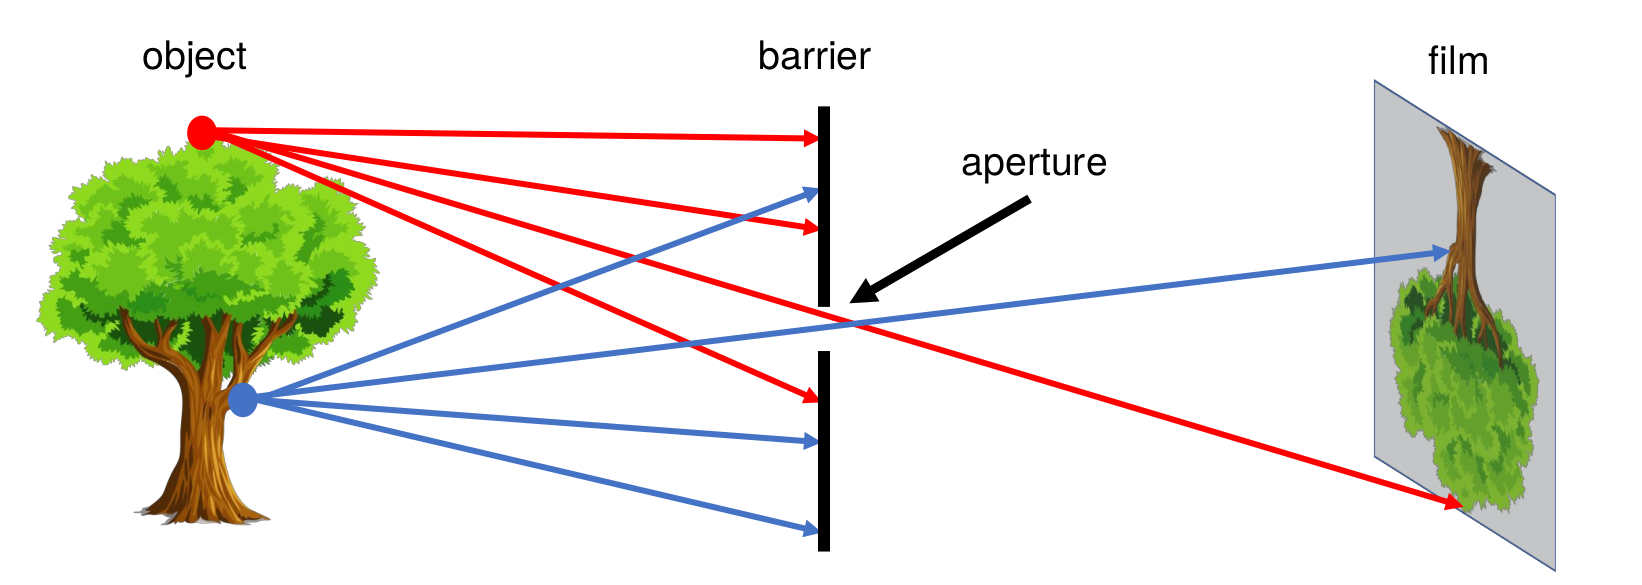
\includegraphics[width=0.6\textwidth]{img/camera/pnhole_effect.png}
	\caption{Pinhole effect on a small aperture. Source:~\cite{camera_models}.}
	\label{fig:pinhole_effect}
\end{figure}

The pinhole camera model describes the perspective transformation on equation~\eqref{eq:camera_transform} as a central projection where all light rays meet at the camera center, $\mathcal{F}_c$. A diagram of the pinhole camera is shown on figure~\ref{fig:pinhole_camera_model}. 

On this model, the z-axis is collinear with the optical axis\footnote{Also called principal axis. The two terms can be changed with no loss of context.}, aligned with the direction the camera is facing. The image plane is at $z = f$, where $f$ is the focal length, being intersected by the optical axis on the principal point, with coordinates $(c_x, c_y)$ on the image plane axis. Note that the principal point is not the origin of the referential on the image plane, but instead the middle point, being the origin located in the top left corner, with a downward y-axis.

\begin{figure}[H]
	\centering
	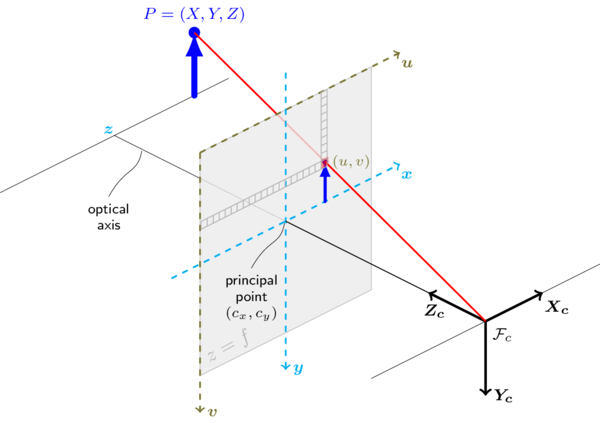
\includegraphics[width=0.6\textwidth]{img/camera/pinhole_camera_model.png}
	\caption{Pinhole camera model. Source: \acl{opencv}~\cite{opencv_doc}}
	\label{fig:pinhole_camera_model}
\end{figure}

Due to the nature of the pinhole camera model, is more convenient to use a Projective Space instead of the more common Euclidean Space~\cite{mvg_book, camera_models, Sturm2010}. On a Projective Space, as in a central camera model, all of its points are oriented through a single point~\cite{mvg_book}. Therefore, by using a projective space instead of a Euclidean for addressing the transformations of a pinhole camera model, mathematics become more intuitive and relatable to the actual geometry of the model. Despite Projective spaces using homogeneous coordinates and non-Euclidean geometry, homogeneous coordinates can be converted for Cartesian coordinates without loss, if the homogeneous points are possible to represent on a Euclidean coordinate frame~\cite{mvg_book, camera_models}.

\subsubsection{Projective Geometry}
A tridimensional Euclidean Space can be represented on a Projective Space using 3+1 coefficients. Therefore, the previous tridimensional vector can be rewritten in homogeneous coordinates as $(wX, wY, wZ, w)$~\cite{mvg_book}. If $w \neq 0$, we can transform from the Projective to Euclidean Space, obtaining the world representation of such points, by dividing the homogeneous point by $w$. For the cases in which $w =  0$, we have purely projective points at infinity, that only exist in Projective Space~\cite{mvg_book}. 

The relation depicted in equation~\ref{eq:camera_transform} can expressed in projective geometry as:

\begin{equation}
	\begin{bmatrix}
		u \\ v \\ 1
	\end{bmatrix}
= P \times 
\begin{bmatrix}
		X \\ Y \\ Z \\ 1
	\end{bmatrix}, \qquad \text{if } w = 1
\end{equation}

$P$ represents the projection matrix that performs the transform from world points to image pixels. The projection matrix in a pinhole camera model is the result of multiplication of two matrices: the camera matrix (or matrix of the camera intrinsic parameters), $K$; and a joint rotation and translation matrix, $[R|t]$ - where $R$ is the rotation matrix and $t$ the translation vector. The combination of these matrices is given on equation~\ref{eq:projective_matrix} and the full camera transform is expanded on equation~\ref{eq:camera_transform_full}, through the replacement of equation~\ref{eq:projective_matrix} in~\ref{eq:camera_transform}.

\begin{equation}
	\label{eq:projective_matrix}
	P = K[R|t]
\end{equation}

\begin{equation}
	\label{eq:camera_transform_full}
	\begin{bmatrix}
		u \\
		v \\
		1
	\end{bmatrix}
	= 
	\overbrace{
		\underbrace{
			\begin{bmatrix}
				f_x & 0 & c_x \\
				0 & f_y & c_y \\
				0 & 0 & 1 
			\end{bmatrix}
		}_\text{\large\textbf{K}}
		\underbrace{
			\left[
				\begin{array}{ccc|c}
					r_{xx} & r_{yx} & r_{zx} & t_x \\
					r_{xy} & r_{yy} & r_{zy} & t_y \\
					r_{xz} & r_{yz} & r_{zz} & t_z 
				\end{array}
		\right]
		}_\text{\large\textbf{[R|t]}}
	}^\text{\large\textbf{P}}
	\begin{bmatrix}
		X \\
		Y \\
		Z \\
		1
	\end{bmatrix}
\end{equation}

The intrinsic parameter matrix is used to represent the calibration parameters of the camera, namely, the focal lengths of each axis, $f_x$ and $f_y$, which scale the $x$ and $y$ axis; the principal point offset to the axis origin, $c_x$ and $c_y$, for the x and y-axis, respectively, that translate the image center with relation to the origin of the camera referential. The joint rotational-translation matrix, $[R|t]$, is also known as the extrinsic camera parameters, translates the coordinates of a point to the Cartesian coordinate system fixed to the camera.


\subsubsection{Cameras, Lenses and Distortion}
Using a simple pinhole for filtering light rays, that would blur the image severely, reduces the amount of light reaching the camera sensor. Therefore, a lens is used to collect the light and focus it onto the image plane, providing the same effects as the hole~\cite{Sturm2010}, while allowing more light to be captured. The paraxial refraction model is represented on figure~\ref{fig:pinhole_with_lense}, from which we can consider the Pinhole Camera model by letting $z_0 = 0$, which implies $z' = f$ and the image is formed on the focal point.

%pinhole effect with a lens is depicted 

\begin{figure}[H]
	\centering
	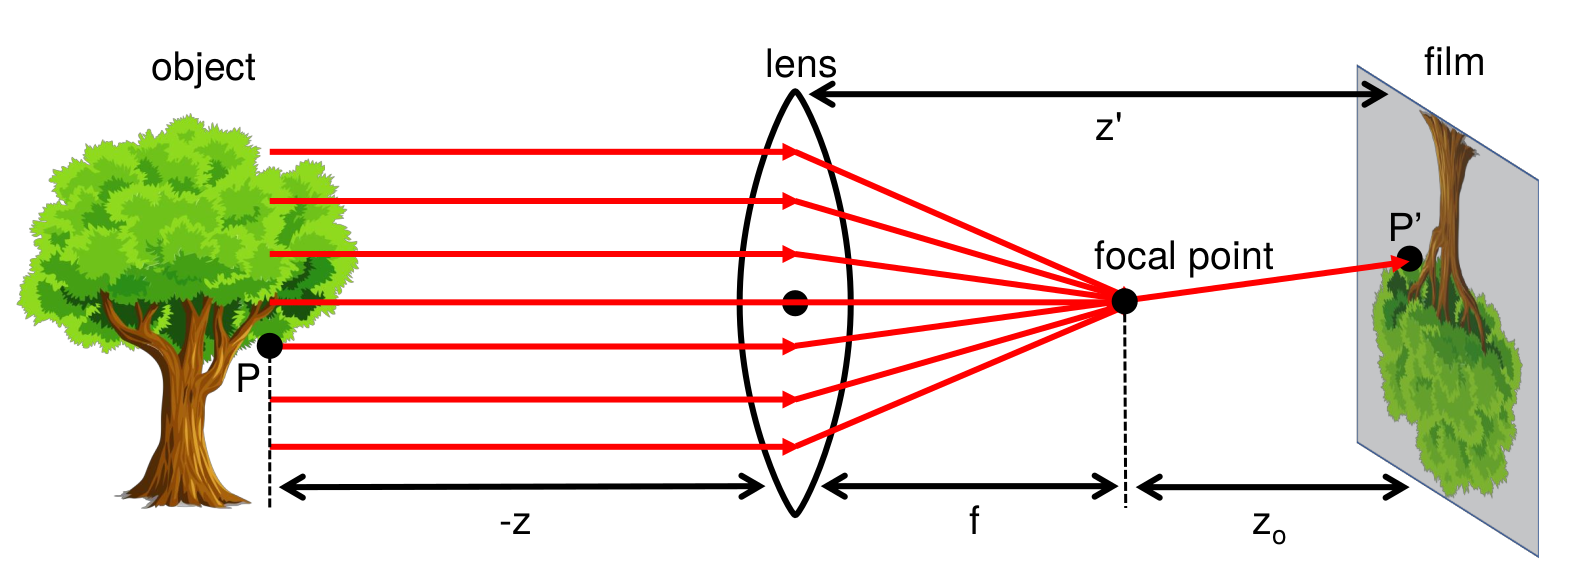
\includegraphics[width=0.6\textwidth]{img/camera/pinhole_with_lense.png}
	\caption{Pinhole effect on a lens. Source:~\cite{camera_models}}
	\label{fig:pinhole_with_lense}
\end{figure}

Since lenses introduce non-linear distortion, the pinhole camera model needs to be extended to included radial and tangential distortion parameters~\cite{Bouguet2010, manuapphotogrammetry, Heikkila1997}. Such parameters indicate how the non-linear distortion of the camera lenses affects the image projection on the camera plane~\cite{camera_models, Sturm2010} and how can this be corrected~\cite{Heikkila1997, Bouguet2010, opencv_doc}. The equations behind that expression are beyond the scope of this introduction and therefore will not be detailed here, but the effect of lens aberration can be seen on figure~\ref{fig:lense_distortion_types}.

\begin{figure}[ht!]
	\begin{subfigure}[c]{0.3\textwidth}
		\centering
		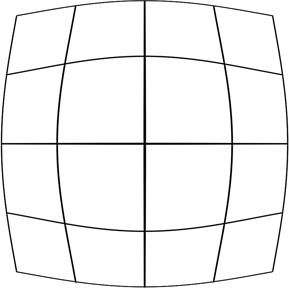
\includegraphics[width=0.6\textwidth]{img/camera/distortion-barrel.png}
		\caption{}
		\label{fig:barrel-distortion}
	\end{subfigure}
	%\quad 
	\begin{subfigure}[c]{0.3\textwidth}
		\centering
		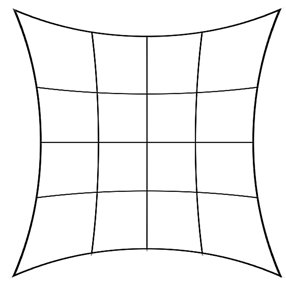
\includegraphics[width=0.6\textwidth]{img/camera/distortion-pincushion.png}
		\caption{}
		\label{fig:pincushion-distortion}
	\end{subfigure}
	%\quad
	\centering
	\begin{subfigure}[c]{0.3\textwidth}
		\centering
		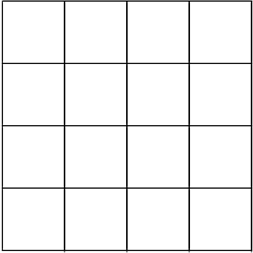
\includegraphics[width=0.6\textwidth]{img/camera/no-distortion.png}
		\caption{}
		\label{fig:no-distortion-lens}
	\end{subfigure}

	\caption{Barrel~(\subref{fig:barrel-distortion}) and Pincushion~(\subref{fig:pincushion-distortion}) distortion caused by the non-linear behavior of the camera lens. The effect of an ideal lens, with no distortion, is shown on sub-figure~(\subref{fig:no-distortion-lens}). Source:~\cite{camera_models}.}
	\label{fig:lense_distortion_types}
\end{figure}

For more information on the pinhole camera model and lens distortion, see Hartley and Zisserman Multi View Geometry in Computer Vision~\cite{mvg_book}, Hata and Savarese course notes~\cite{camera_models} or \acf{opencv} official documentation~\cite{opencv_doc}. 

\subsection{Camera Intrinsic Calibration}
\label{subsec:sota:camera-intrinisc-calibration}
Calibrating a camera is the process on which the parameters of the model that describes its behavior are determined. For the extended pinhole camera model, this means determining the parameters of its intrinsic matrix, $K$, but also the distortion coefficients of the lens used~\cite{mvg_book, camera_models, Bouguet2010, Heikkila1997}. These parameters are called the intrinsic parameters and are independent of the scenario being viewed, if the focal length is kept constant. On the other hand, extrinsic camera parameters are different for every situation and therefore scenario dependent~\cite{opencv_doc, Bouguet2010, Heikkila1997}.

Zhang proposed in 2000 a method for calibrating a camera that unlike previous others, does not require a special setup, expensive experimental apparatus or complicated calibration patterns: it uses a planar object with a known pattern, which can be freely moved in front of the camera~\cite{Zhang2000}. Only two images are necessary for camera calibration, as long as the pattern movement between them is not a pure translation. The estimation of the camera intrinsic parameters and distortion caused by the lenses can be determined by solving the equation~\ref{eq:camera_transform_full}, once several $2D \leftrightarrow 3D$ correspondences have been established.

Zhang's algorithm differs from other algorithms at the time that attempted to calibrate a camera by rotating it on a static environment. Other alternatives include Tsai's algorithm~\cite{Roger1987, mvg_book}, a 2-stage technique for camera calibration first presented in 1987, that does not determine the camera center. A \ac{dlt} algorithm can also be used to determine the camera calibration parameters (see~\cite{mvg_book}).

Following Zhang's algorithm, the correspondences between the 2D and 3D representations of the pattern can be made by finding the corners or circles on planar patterns~\cite{opencv, mvg_book}. Chessboards are the most common patterns used today~\cite{opencv}, allowing corner detection for each cell (figure~\ref{fig:opencv_calib_pattern}). Since the dimensions of the cell and their arrangement are known previously, it is possible to compute the orientation of the chessboard~\cite{Zhang2000, opencv_doc, mvg_book}. On those conditions, revisiting equation~\eqref{eq:camera_transform_full}, only the $K$ matrix is left to be determined. 

\begin{figure}[t]
	\centering
	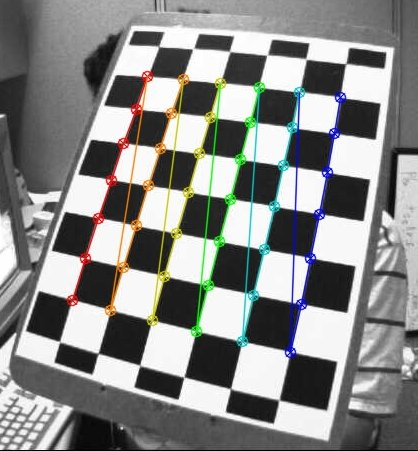
\includegraphics[width=0.4\textwidth, keepaspectratio]{img/camera/calib_pattern.jpg}
	\caption{Chessboard calibration pattern with corners detection results show on image. Corner order is also given on the corner color. Source:~\cite{OpenCV_camera_calib}.}
	\label{fig:opencv_calib_pattern}
\end{figure}

The intrinsic calibration matrix coefficients can then be refined using a maximum-likelihood estimation to minimize the error using a non-linear method, such as Levenberg-Marquardt optimization~\cite{Levenberg1943}. Other optimizations are possible, such as Powell’ dog-leg non-linear least squares technique~\cite{Lourakis2005}. Further reading can be conducted on~\cite{mvg_book, Sturm2010, camera_models, Hata, Xu1996a}.

Bouguet in 2010 provided a Camera Calibration toolbox for \ac{matlab}~\cite{Bouguet2010}, which serves as the basis for many camera calibration toolboxes nowadays, such as \ac{opencv}, which is also based on the work of Zhang~\cite{opencv}.

\subsection{Image Processing Libraries for \acl{cv}}
In the field of computer vision, several tools and libraries are available, capable of performing low image operations, image detection, filtering, among others. 

\begin{itemize}
	\item \textbf{BoofCV~\cite{boofcv}:} written in Java, this library is oriented to real-time image operations, such as low-level image processing, camera calibration and feature/object  detection, tracking and recognition;
	\item \textbf{Dlib~\cite{dlib}:} modern C++ toolkit containing \acl{ml} algorithms and tools, some on the field of computer vision;
	\item \textbf{\ac{matlab} Computer Vision Toolbox\texttrademark~\cite{matlabcvtoolbox}:} toolbox for computer vision algorithms, 3D vision, and video processing systems. Can perform object detection and tracking. Detects, extracts and matches features;
	\item \textbf{\acf{opencv}~\cite{opencv}:} open source library for C++, Python and C that implements the state of the art algorithms on computer vision;
	\item \textbf{Vlfeat~\cite{vlfeat}:} open source library for C that implements many state of the art algorithms on computer vision;
	\item \textbf{SimpleCV~\cite{simplecv}:} Open source framework, written in Python, that can be used to implement computer vision software using other libraries;
\end{itemize}

Since a goal of this work is to use Open-Source tools as far as possible (instead of using closed source tools or code that is harder to integrate with other libraries), which is common among the automotive industry on the field of autonomous vehicles, \ac{matlab} \acl{cv} Toolbox\texttrademark~does not suit. The code of this work is mainly developed in C++, so Python and Java libraries will not be considered, resulting only in \ac{opencv} and Dlib (Vlfeat uses plain C, so its not suited). 

\ac{opencv} has a large and active community and is considered by many researchers and industry leaders as the \textit{de facto standard} library when refereeing to computer vision. Dlib is a robust library, but no significant differences can be seen when comparing with \ac{opencv}. Therefore, the final choice for a computer vision library is \ac{opencv}, also because of the already implemented compatibility with \ac{ros}.



%%%%%%%%%%%%%%%%%%%%%%%%%%%%%%%%%%%%%%%%%%% LIDAR %%%%%%%%%%%%%%%%%%%%%%%%%%%%%%%%%%%%%%%%%%

\section{Automotive \ac{lidar}}
\label{sec:sota:automotive-lidar}
\ac{lidar} sensors map their surroundings thanks to their high spatial resolution and capability of precisely measuring depth. Already used in topography, spectrography and air pollution studies, \ac{lidar} found its importance on the automotive industry as one of the key sensors of autonomous cars and \ac{adas}~\cite{Sullivan2016}. 

The maps produced by the \ac{lidar}, commonly represented as point clouds or mesh clouds models, (see figure~\ref{fig:bunny}), are one of the preferred method for \ac{slam} algorithms, which allow a vehicle without previous knowledge of its surroundings to autonomously navigate them, a crucial task for \ac{adas} on self-driving vehicles.

Point clouds represent the spatial data measured by the \ac{lidar} as points on the tridimensional space. The objects represented on a point cloud are formless, as they have no relation with their ``adjacent'' points, as depicted on sub-figure~\ref{fig:bunnyPointCloud}. A Mesh cloud representation of the point cloud on sub-figure~\ref{fig:bunnyMeshCloud}, produced from by the point cloud on sub-figure~\ref{fig:bunnyPointCloud}, is a representation of the same points united by lines, forming a mesh. A mesh cloud conveys form, as can be verified by comparing the point cloud with the mesh representation of the same data. A mesh cloud, contrary to a point cloud, can also represent a close form and therefore having a volume.

\begin{figure}[!ht]
	\centering
	\begin{subfigure}[c]{0.45\textwidth}
	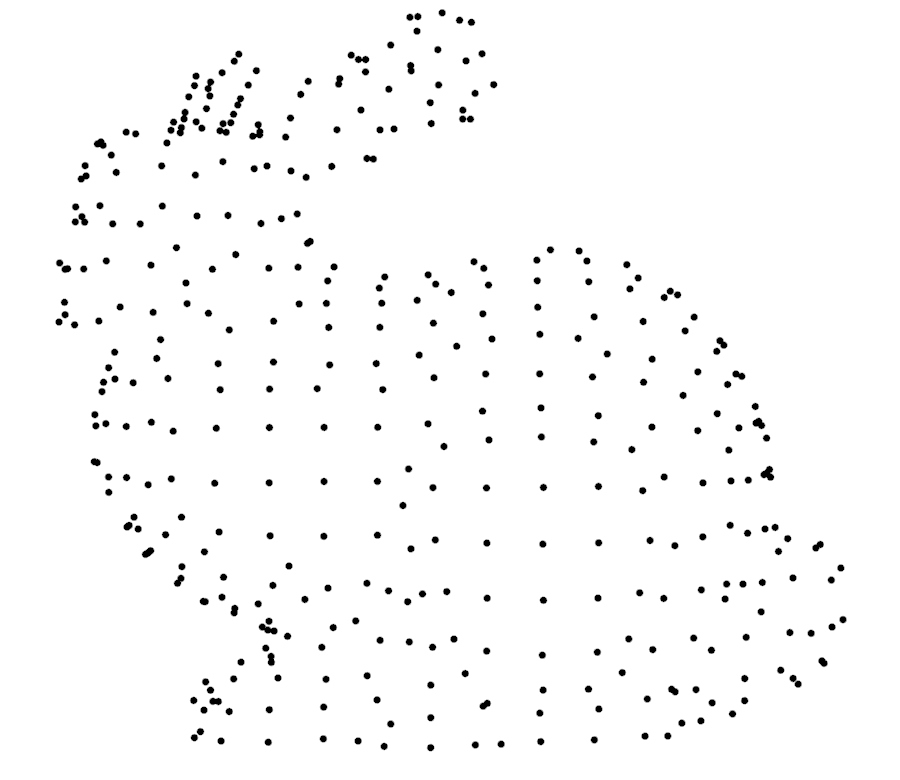
\includegraphics[width=\textwidth]{img/lidar/bunny_point.png}
		\caption{Point Cloud representation}
		\label{fig:bunnyPointCloud}
	\end{subfigure}
	\quad
	\begin{subfigure}[c]{0.4\textwidth}
		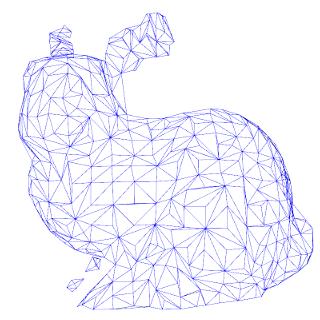
\includegraphics[width=\textwidth]{img/lidar/bunny_mesh.png}
		\caption{Mesh Cloud representation}
		\label{fig:bunnyMeshCloud}
	\end{subfigure}
	\caption{Stanford bunny~\cite{bunny} point cloud (\subref{fig:bunnyPointCloud}) and mesh cloud (\subref{fig:bunnyMeshCloud})}
	\label{fig:bunny}
\end{figure}

\subsection{\ac{lidar} classification based on the depth measurement principle}
Regarding the type of signals and principles for measuring the scene distance, \acp{lidar} can be either \ac{cw} (emit a sinusoidal or square modulated signal), pulsed (emit a square pulse at fixed moments in time)~\cite{Payne2009, TexasLiDAR, SpringerOptics} or other more exotic and experimental types, that will not be addressed here.

\ac{cw} \acp{lidar} continuously emits a modulated laser signal to their surroundings and, depending on the modulation technique, this signal can either be \ac{am} or \ac{fm}\cite{TexasLiDAR}. \ac{am}\ac{cw} \acp{lidar} operates by emitting a pseudo-random stream of binary data and coherently detecting the received signal. The phase shift distance, measured between the emitted and received signal, is directly related with the distance at which the pulse was reflected.

If \ac{fm}\ac{cw} is used instead, the \ac{lidar} \ac{laser} sends a frequency chirp\footnote{A signal whose frequency varies linearly with time.} and coherently detects the received signal, estimating the distance at which the reflection occurred (i.e., the object is), by the frequency shift between the emitted and reflected signals\cite{Payne2009, TexasLiDAR}. Coherent detection can be performed by heterodyne or homodyne detection, but such details will not be addressed here. A brief description and comparison between the two detection modes applied to \ac{lidar} technology is given here~\cite{Conroy2009}, and the underlying theory can be consulted on~\cite{Carlson2010, SpringerOptics}.

Pulsed \ac{lidar} technology acquires depth information by measuring the \acf{tof} between the reflection and emission of the same light pulse by the \ac{lidar} \ac{laser}. This technology is the most common type used for measuring depth on automotive \ac{lidar}~\cite{Sullivan2016}, and therefore this work will be based on pulsed~\ac{tof} technology to measure the distance at which the obstacles on the scene are present.

Both \ac{cw} and \ac{tof} \ac{lidar} have advantages and disadvantages, but they will not be compared here. Further reading about the topic can be continued on~\cite{Sullivan2016, Simonite2017, Payne2009, TexasLiDAR}.


\subsection{\ac{lidar} classification based on construction}
Despite the depth measurement technique used by the \ac{lidar} device, regarding its construction and mapping technology, automotive \acp{lidar} can be one of the following categories~\cite{Hecht2018, Sullivan2016}:

\begin{enumerate}
	\item \textbf{Rotating \ac{lidar} or Macro-scanners:} the most common type, the \ac{lidar} optical and electrical circuit are mounted on a mechanical rotating device, which normally results on a wider \ac{fov} than the other models~\cite{Sullivan2016};
	\item \textbf{Flash:} organized in a matrix structure, similar to a camera \ac{ccd}, every element of the matrix contains a photodetector. A ``flash'' simultaneous illuminates all the \ac{fov}, and the reflected light intensity and time of arrival is measured to provide depth calculations, in simultaneous for all pixels of the depth image~\cite{TetraVue, Ouster, Gelbart2002,Stettner2010, Simpson2019}; 
	\item \textbf{\ac{mems}:} operate by controlling the angle at which a rotating microscopic mirror is aligned with the \ac{laser}. By varying the angle a single line can be scanned and using multiple \acp{laser} with the same mirror allows vertical scan~\cite{LeddarTech, Yoo2018};
	\item \textbf{Phased Arrays:} still on an embryonic stage, phased array \ac{lidar} use a microscopic array of antennas, similar to a \ac{radar}, where the phase of each antenna is individually controlled to allow the \ac{lidar} to sweep and/or focus on a specific area, using beamforming theory~\cite{Quanergy2018, Yu2016}.
\end{enumerate}

Of all the four types of \ac{lidar} presented, \ac{mems} and phased array \ac{lidar} are still unsuited for autonomous vehicles, since they have yet to leave their early research state and develop a functional prototype~\cite{Sullivan2016, Hecht2018}. 

Flash \ac{lidar}'s, also referred by some authors as solid state \ac{lidar}, since it was no movable parts, has the potential to become the most reliable, durable and cheaper \ac{lidar} technology~\cite{Sullivan2016, Hecht2018, Fersch2017a}. However, this technology is not yet mature, with some of its best experimental  prototypes achieving a maximum distance of \SI{2}{\meter}~\cite{Hecht2018}. The main cause for such lower range is the attenuation of the flash intensity, since its power is inversely proportional with the distance squared.

Some prototypes are also unveiled from startups, such as TetraVue~\cite{TetraVue} and Ouster~\cite{Ouster}, and some patents are being registered~\cite{Simpson2019}; but this \ac{lidar} technology is not yet suited for the automotive market of autonomous cars~\cite{Fersch2017a}.

Therefore, only one alternative remains: a mechanical rotating \ac{lidar}, which is the technology that will be chosen for this work.

\subsection{The Mechanical Rotating \ac{lidar}}
To construct a rotating \ac{lidar}, a single pair of \acp{laser} and photodetectors are assembled on a fast rotational device (typically \SIrange{5}{20}{\revspersecond}), allowing that pair to scan a single line while rotating, creating a 2D \ac{lidar}. If multiple pairs are assembled with different polar angles, the \ac{lidar} is said to be a 3D \ac{lidar}, since a total revolution can produce a three-dimensional map of its surroundings~\cite{Sullivan2016}.

While a rotating \ac{lidar} consumes more power than the other counterparts, it can also achieve ranges until 100 meters~\cite{vlp16, Sullivan2016} or even 200 meters~\cite{VelodyneHDL64, Pandar40UserGuide, Sullivan2016}. To measure the depth on a rotational \ac{lidar}, \ac{tof} is the most common technique, being the pulse triggered at a defined angular step when rotating.

Regarding rotating \acp{lidar} technology only 5 relevant companies exist worldwide. Velodyne\cp~\cite{Velodyne}, HESAI\cp~\cite{Hesai}, RoboSense\cp~\cite{Robosense}, Ouster\cp~\cite{Ouster} and Quanergy\cp~\cite{Quanergy}. Velodyne is the undisputed market leader~\cite{Sullivan2016, Hecht2018}, with several rotating \ac{lidar} solutions, ranging from \SIrange{16}{128} laser beams.

Quanergy is a \ac{lidar} company that is focused on bringing solid state \ac{lidar} to the market. They provide on mechanical rotation \ac{lidar} solution, but with only 8 beams, which is not suited for the demands of autonomous driving~\cite{Sullivan2016, Hecht2018}. 

Ouster is a startup that produces mechanical rotational \acp{lidar}. They have two models, \texttt{OS-1} and \texttt{OS-2}, for mid and large range, respectively, which differ on their \ac{fov}, range and number of beams~\cite{Ouster}.

HESAI and RoboSense are two Chinese \ac{lidar} manufacturers whose products are similar to Velodyne's. In fact, they are so similar that a lawsuit as been filled against them by Velodyne, for intellectual property issues~\cite{VelodyneLawsuit}. This lawsuit is due to Velodyne holding the patent on mechanical rotating \acp{lidar} with surround view\cite{Hall2011}, which ensures its dominance on the market of mechanical \ac{lidar}. 

In fact, on their specifications, \acp{lidar} from Velodyne, HESAI, RoboSense or Ouster differences are laser position managing, range and vertical \ac{fov}. On the other hand, they severely differ in terms of prices, with top of the range Velodyne \ac{lidar} selling for $\$85000$ and the cheaper at some thousand dollars. 

For our work, since Velodyne's is the top of the market solution and the more mature, it makes sense to test \ac{lidar} interference on the most used solution, since if two \acp{lidar} will interfere on the road, the most likely scenario is that they are from Velodyne's.

\subsection{Point Cloud Processing Software}
Excluding software that is developed for the final user, and not for a developer, VeloView\texttrademark, a \ac{lidar} data visualizer by Velodyne is excluded as an alternative for this thesis, since it only allows to visualize data and save/load data from files. Similarly, programs that only intend to provide some features to apply to point clouds, and do not allow for research on point cloud processing to be conducted, are not viable solutions for this work. 

From the software that as not being excluded by the conditions above, several point cloud processing libraries were researched: 

\begin{itemize}
	\item \textbf{\ac{gcal}:}	a library containing geometric algorithms, written in C++, optimized for polygons and polyhedra processing, that is target for geographic information systems, such as computer aided design, molecular biology and robotics, among others\cite{GDAL};
	\item \textbf{\ac{pdal}:} written in C++, \ac{pdal} is an adaptation of \ac{gcal} optimized to handle point cloud data. It is more oriented for the user to define a process pipeline in JavaScript, from already available algorithms on its library than for the developer to implement its own\cite{PDAL};
	\item \textbf{Open3D:} written in C++, Open3D is a library optimized for common operation in point cloud processing, providing voxelization, nearest neighbor search, normal estimation and visualization interfaces, among other utilities~\cite{Open3D};
	\item \textbf{\acf{pcl}:} Open-Source and with an active community, \ac{pcl} is a large library for 2D/3D image processing and point cloud processing. It allows generic data types, has a comprehensive amount of state of the art algorithms and easily integrates with \ac{opencv} and \ac{ros}~\cite{PCL}.
\end{itemize}

All the alternatives are written in C++, the programming language of choice for this work. From the 4 libraries, \ac{gcal} is not optimized for point cloud data and \ac{pdal} intends to simplify routine point cloud processing, which is not aligned with the objectives of this thesis, reason why we exclude them both. Open3D and \ac{pcl} are reasonable alternatives, but \ac{pcl} modularity (allowing the user to define its data types) and extent of already implemented algorithms makes it a better solution than Open3D. Since we will also use \ac{opencv} and \ac{ros}, which \ac{pcl} allows integration and this topic is widely detailed on forums, our choice for a point cloud processing library is \ac{pcl}.

\section{Camera and \ac{lidar} Extrinsic Calibration}
\label{sec:sota:extrinsic_calibration}

On a multiple sensor setup, coordinated frames from one sensor must be able to be referred on another sensor coordinate frame. Transforming data from one frame to another requires performing extrinsic calibration between them by determining the rigid body transform that can convert the data from one reference plan to the other without loss of information.

Therefore, the sole purpose of extrinsic calibration is to determine the coefficients of this transform, that can be described as a rotation and a translation, similarly to the joint rotation-translation matrix $[R|t]$ used for camera intrinsic calibration (equation~\ref{eq:camera_transform_full}). However, on this case, instead of this matrix representing the rotation of the object to the camera or the camera movement in the world, it represents the rotation and translation operations that need to be applied to the coordinate system of one sensor (and its data) to align the data with the coordinate system of another sensor. The precision of this transformation takes particular interest when data fusion (or sensor fusion) is being achieved, i.e., merging from this data sources to reduce errors and improve the significance of data each sensor is capable of giving. 

Several algorithms have been suggested for performing extrinsic calibration on data. They range from the necessity of well controlled environments to requiring no human intervention, using or not a calibration pattern. 


\subsection{Calibration using Patterns}
Typical extrinsic calibration between \ac{lidar} and camera with intersecting \ac{fov} use calibration patterns: Unnikrishnan first proposed a \ac{lidar}-Camera extrinsic calibration using a toolbox developed to manually select correspondences between a calibration pattern on image and point cloud~\cite{Unnikrishnan2005}. A \ac{matlab} toolbox to ease the process was also been developed in 2005 by Unnikrishnan\etal~\cite{Unnikrishnan}. Fremont\etal uses a planar calibration target with a hole surrounded by a solid color, matching the depth discontinuities from the \ac{lidar} with the color discontinuities from the camera~\cite{Fremont2013} and Velas uses a planar pattern with geometric objects carved on its surface~\cite{MartinVelas2013}. Liao\etal proposes a method that only requires the usage of a planar polygon of known shape~\cite{Liao2019} and Park\etal tests and presents results of this calibration method applied to multiple polygons, specially with triangular shape~\cite{Park2014}. Mirzaei\etal uses a planar pattern with fiducial marker~\cite{Mirzaei2012}. 

Regarding calibration with three-dimensional calibration targets, Pusztai uses a box with different colors on each face~\cite{Pusztai2018}; Pereira a ball (for performing multiple sensor calibration, instead of only 3D \ac{lidar} and monocular camera)~\cite{Pereira2016}; Gong a trihedral object, determining the extrinsic calibration parameters using a nonlinear least squares algorithm~\cite{Gong2013}.

While the previous methods where focused on calibrating monocular cameras with tridimensional \ac{lidar}, alternative methods exist for stereo systems, taking advantage of the disparity map obtained with a stereo camera. Automatic methods are proposed by Geiger\etal and Guindel \etal. Geiger\footnote{One of the researchers behind \ac{kitti}.} and Moosmann propose a method for calibrating such setup with a single shot, using chessboards with multiple sizes and orientations. Their algorithm initializes seed point on the chessboard corners on image, and by region growing algorithms detects the chessboard position on camera, while on \ac{lidar}, planar detection and successive refinement is applied~\cite{Geiger2012a}. Guindel\etal use a planar calibration target with four holes that can be detected on the stereo map from the camera and \ac{lidar} point cloud, extrinsically calibrating both sensors by detecting the holes center and compute the rotation and translation that minimizes error. 

\subsection{Calibration without human intervention or patterns}
Some automatic methods that do not require human intervention neither calibration patterns have also been present on the literature. Bileschi's method estimates all intrinsic camera parameters  (including radial distortion) and the rotation and translation between a camera and \ac{lidar}, that is later refined by discontinuity association~\cite{Bileschi2009}. Naroditsky \etal proposes an automatic calibration method using the multi-polynomial Macaulay resultant, that, paired with \ac{ransac} and least-squares refinement, can automatically calibrate the camera-\ac{lidar} setup~\cite{Naroditsky2011}. Shaukat proposes a solution for planetary space robots based on  stereopsis and depth maps matching using mesh grids stecthing~\cite{Shaukat2016}. Ishikawa \etal calibration method, computes the calibration parameters using two main steps: first, initializes the parameters from the movement of the camera and \ac{lidar} and secondly, refines the parameters using sensor-fusion until convergence~\cite{Ishikawa2018}. 

Jeong \etal presents a framework for calibrating \ac{lidar} and stereo cameras with non-overlapping \ac{fov}, by utilizing road markings and robust optimization algorithms and cost functions~\cite{Jeong2019}.

Using mutual information techniques, Taylor and Nieto's approach uses normalized mutual information between camera and \ac{lidar}, maximizing the features to be matched on a particle swarm map, with refinement techniques~\cite{Taylor2013}; Pandey's \etal approach defines a cost function for the mutual information and using known methods, minimize and refine the results to obtain the best parameters~\cite{Pandey2012}.


\subsection{Other calibration methods}
Other calibration techniques use data variation through time~\cite{Chien2017} or Deep learning on \ac{cnn}~\cite{Wang2018a}. Scaramuzza \etal introduce a simple technique for extrinsic calibration that does need calibration patterns~\cite{Scaramuzza}: instead it requires the user to manually select correspondences between the camera and \ac{lidar}, easing the selection with the transformation of point clouds to Bearing Angle images. Brabec offers advances on this method, using a semi-automatic process where correspondences between the camera and \ac{lidar} (presented as a directional image) data are selected by the user and refined using local correction and \ac{ransac} algorithms~\cite{brabec2014}.

Varuna De Silva \etal propose an approach based on the geometric positioning of the sensors on the setup, determining the parameters through geometric description between them, later refining this estimate using depth maps and a non-linear refinement technique (Gaussian Process Regression)~\cite{DeSilva2018}. In another of their works, a planar calibration pattern with holes is used, followed by the same refinement technique~\cite{Silva2018}.


\subsection{Summary of Extrinsic Calibration Techniques}
Multiple calibration techniques were described on this section, with some requiring special calibration patterns, others do not need even require human intervention and some of them rely on deep learning and \ac{nn}. 

Extrinsically calibration between the \ac{lidar} and camera, if performed using a pattern,  requires the calibration object to contain relevant information to both the camera and the \ac{lidar}. A calibration pattern with relevance to the camera implies having a color or a known pattern. For the \ac{lidar}, depth discontinuities are required. In order to create a good calibration pattern with depth discontinuities, either it is bulky or the depth discontinuity is caused by a hole and therefore the distance to the background varies. Either way, such calibration method is not practical, therefore will not be used.

Relying on \ac{nn}, time variation or other exotic techniques will only add unnecessary complexity to this work, which would deviate us from the intended goals. Fully automatic methods would also require a large amount of time to implement, validate and tune to the experimental setup data, which is impractical.

From all the methods presented, our efforts will be placed on a semi-automatic solution, with refinement, that requires user interaction and then refines the calibration parameters estimated. Examples of such work are Taylor and Nieto's~\cite{Taylor2013}, Pandey's~\cite{Pandey2012},Scaramuzza~\cite{Scaramuzza}, Brabec~\cite{brabec2014} and Varuna~\cite{DeSilva2018}.


\section{Sensor Fusion}
\label{sec:sota:sensor-fusion}
Fusing sensory data is the task of combining different data formats, acquired by different sensors into a multi-modal view of the world. This multi-modal view not only allows a better interpretation of the individual data, but also allows the raise of higher context semantics, since fused data is more than the sum of its parts.

Sensor data needs to be preceded by proper extrinsic sensor calibration before data can be fused. For monocular RGB cameras and \ac{lidar}, sensor fusion translates to augmenting the depth information of a point cloud by adding color from the image obtained with the camera or overlapping on the camera image the distances at which objects appear on \ac{lidar} data. An example of a colored point cloud (retrieved from~\cite{Gong2013}) can be seen on figure~\ref{fig:colored_point_cloud_example} and an image overlapped with \ac{lidar} distance measurements (retrieved from~\cite{Bileschi2009}) can be seen on figure~\ref{fig:image_with_lidar_distance}.

\begin{figure}[!ht]
	\centering
	\begin{subfigure}[t]{0.55\textwidth}
		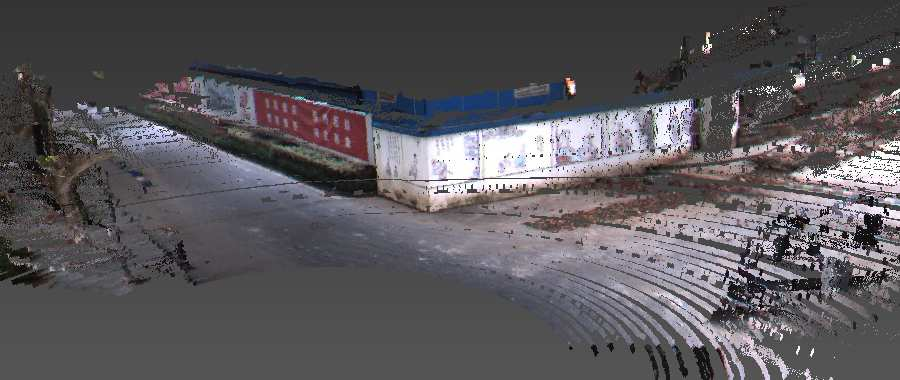
\includegraphics[width=\textwidth]{img/sensor_fusion/colored_point_cloud.png}
		\caption{Colored Point Cloud. Source~\cite{Gong2013}}
		\label{fig:colored_point_cloud_example}
	\end{subfigure}
	\quad
	\begin{subfigure}[t]{0.40\textwidth}
		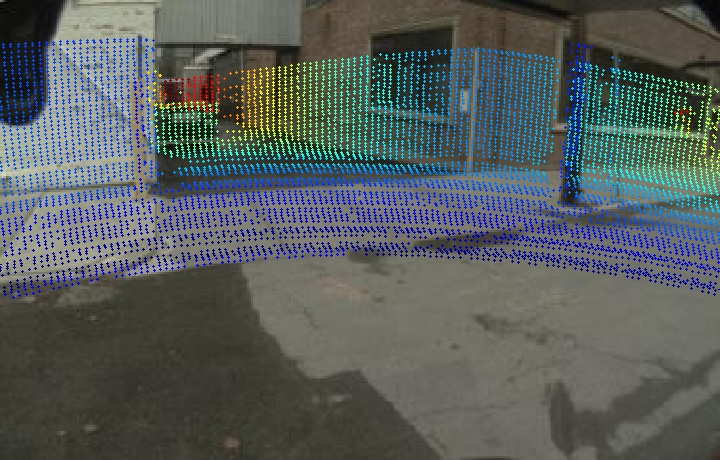
\includegraphics[width=\textwidth]{img/sensor_fusion/image_with_distance_point_cutted.png}
		\caption{Camera Image with overlapping distance measurements. Source~\cite{Bileschi2009}}
		\label{fig:image_with_lidar_distance}
	\end{subfigure}
	\caption{Examples of sensor fusion between camera and \ac{lidar}. Sub-figure~(\subref{fig:colored_point_cloud_example}) represents a colored point cloud, whose pixels are projected to the point cloud and nearby 3D points are colored with the color of their correspondent pixel. Since \ac{lidar} \ac{fov} is wider than the camera's, several points are black because no correspondences can be made. Sub-figure~(\ref{fig:image_with_lidar_distance}) displays an image with overlapping distance measurements. Point cloud points in the image \ac{fov} are projected into the image and color mapped with intensity.}
	\label{fig:point_cloud_camera_fusion_example}
\end{figure}

There are tree major types of sensor fusion: 

\begin{enumerate}
	\item \textbf{Calibration + Fusion:} Sensors are first calibrated among themselves, using one of the techniques described on section~\ref{sec:sota:extrinsic_calibration}, and then data is converted to a referential of choice and merged;
	\item \textbf{Simultaneous Calibration and Fusion:} the implemented algorithms attempt to merge the data by minimizing an appropriated cost function. The final result consists on the multimodal merged data and the calculated extrinsic calibration parameters;
	\item \textbf{``Direct'' Sensor Fusion:} Genetic algorithms, neural networks or other similar tools analyze \ac{lidar} and camera data, without knowing any previous information about them, and output the merged data in the desired format.
\end{enumerate} 


\subsection{Calibration + Fusion}
\label{subsec:sota:calibration-and-fusion}
After calibrating the camera and \ac{lidar}, the data from these sensors can be fused, for a visual assessment of the correctness of the calibration. Some authors' whose work is referred on section~\ref{sec:sota:extrinsic_calibration}, also show the results of sensory fusion applied to their data with the results of the proposed calibration algorithms, as a proof of calibration correctness. Unnikrishnan\etal~\cite{Unnikrishnan2005}, Velas\etal~\cite{MartinVelas2013}, Mirzaei\etal~\cite{Mirzaei2012}, Pusztai\etal~\cite{Pusztai2018} and Gong\etal~\cite{Gong2013} opt to use the camera information to color the point cloud, showing a colored point cloud (for Gong's\etal example, refer to sub-figure~\ref{fig:colored_point_cloud_example}). Others, such as Fremont\etal~\cite{Fremont2013}, Liao\etal~\cite{Liao2019} and Park\etal~\cite{Park2014} prefer to show a visual metric of the calibration correctness by overlapping depth information gathered by the \ac{lidar} onto the image.

This sensor fusion technique is based on the application of the affine transformation described in equation~\eqref{eq:jointRotationTranslationTransform}, which transforms data from the \ac{lidar} coordinate frame to the camera, allowing for a $3D point \leftrightarrow pixel$ mapping, enabling either point cloud coloring or overlapping the distance measurements on the image, as previously shown in figure~\ref{fig:point_cloud_camera_fusion_example}.
	
\begin{equation}
	\label{eq:jointRotationTranslationTransform}
	\begin{bmatrix}
		X_{cam} \\
		Y_{cam} \\
		Z_{cam} \\
		1
	\end{bmatrix}
	= 
		\underbrace{
	\left[
			\begin{array}{ccc|c}
				r_{xx} & r_{yx} & r_{zx} & t_x \\
					r_{xy} & r_{yy} & r_{zy} & t_y \\
					r_{xz} & r_{yz} & r_{zz} & t_z \\
					0      & 0      & 0      & 1 
				\end{array}
		\right]
		}_\text{\large\textbf{[R|t]}}
	\begin{bmatrix}
		X_{LiDAR} \\
		Y_{LiDAR} \\
		Z_{LiDAR} \\
		1
	\end{bmatrix}
\end{equation}


\subsection{Simultaneous Calibration and Fusion}
\label{subsec:sota:simultaneous-calibration-fusion}
Li\etal proposes a method for simple indoor setups consisting of a single camera and a \ac{lidar} on a servo motor. The mechanism is rotated for three angular positions and a point cloud and image is taken for each one. Then, every image and point cloud are stitching together using fiducial features, resulting on a colored point cloud and on the determination of the calibration parameters~\cite{Li2016}. 

Park\etal also proposes a method for fusing uncalibrated \ac{lidar} and stereo camera data, using two \ac{cnn}: one for calibration, by reducing error between disparity images; and a second to refine the fused disparity maps with the left image~\cite{Park2019}. 

Yang\etal also proposes a method for stereo image and \ac{lidar} point cloud fusion using a Generalized \acl{icp} algorithm to match features and extracted a fused tridimensional refined model, at the same time it estimates the rigid body transform between camera and \ac{lidar}~\cite{Yang2017}.

Castorena\etal approach for sensor fusion matches the edges using a weighted total variation norm, fusing depth maps from a \ac{tof} camera with \ac{lidar} point clouds, useful not only for calibration, but also to refine the results of the fusion process and generate a more accurate colored point cloud~\cite{Castorena2016}.

\subsection{``Direct'' Sensor Fusion}
Still on embryonic steps, ``direct'' sensor fusion relies on deep learning to learn how to calibrated and fuse \ac{lidar} and camera data, therefore not requiring any previous knowledge about the dataset. It differs from sub-Section~\ref{subsec:sota:simultaneous-calibration-fusion} because the features and the cost function to be minimized are determined by the neural network and not projected by the researchers.

Liang\etal approach uses a multi-task multi-sensor dense fusion network for camera and \ac{lidar} fusion, that can not only fuse the data and creating a colored point cloud, but also perform object detection on image and point cloud, with 3D bounding box estimation~\cite{Liang2019}.

Wei\etal research is aimed for a real-time multi-sensor collision avoidance system, on which the standalone usage of camera and \ac{lidar} does not yield satisfactory results~\cite{Wei2018}. The sensor fusion algorithm uses a \ac{cnn} and feature extraction to fuse \ac{lidar} and camera data. 

\subsection{Considerations about the different methods and our work}
On our work, since we are aiming to first calibrate the sensors and then fuse the data, following a more ``traditional'' approach to sensory data fusion, our algorithm will be based on the methods described in sub-Section~\ref{subsec:sota:calibration-and-fusion}. 

Simultaneous calibration and fusion methods (sub-Section~\ref{subsec:sota:simultaneous-calibration-fusion}) would be interesting, but the research focus to develop one of those methods would deviate our work from the \ac{lidar} interference study.

On the alternatives that rely on neural networks and deep learning, Wei\etal~\cite{Wei2018} solution is attractive, but it was only published on June, which impossibilities its usage on this work.

\section{Object Detection}
\label{sec:sota:object-detection}

Object Detection is a field of \acl{cv} that intends to detect objects in image. Currently, two approaches to tackle this problem are possible:

\begin{enumerate}
	\item \textbf{\acl{ml} based approach:} objection detection is performed on two steps: first a set of feature descriptors are chosen and extracted from reference images; secondly a \acf{nn} takes those features and perform the classification;
	\item \textbf{Deep-Learning based approach:} end-to-end object detection without the need of handmade feature engineering.
\end{enumerate}

\subsection{\ac{ml} based approach}
When referring to the first solution, Haar-like features~\cite{Messom2006}, \ac{sift}~\cite{Hughes2011a}, \ac{surf}~\cite{Bay2008} and \ac{hog} features~\cite{Dalal2010, Surasak2018} are normally used, on a Viola-Jones \ac{nn} (or its extensions)~\cite{Viola2001, ViolaP2004}. % For more details see 

\subsection{Deep-Learning based approach}
The second solution is normally implemented with a Region Proposal \acf{cnn}, developed by Girshick\etal on 2014~\cite{Girshick2014}. A common \ac{cnn} cannot be used for object detection on an image because the number of detected objects is variable, and so would the size of the output layer need to be, which is not possible on this architecture. A \ac{rcnn} differs from a \ac{cnn} due to the region proposal algorithm preceding it, that limits the number of regions to be evaluated on an image to approximately 2000, therefore limiting the number of objects on an image~\cite{Girshick2014}. However, this \acl{nn} needs to be run for every one of the 2 thousand regions, making it slow and infeasible for real-time object detection~\cite{Girshick2014}. One year later, Girshick proposed a new architecture called Fast \ac{rcnn}, that runs the convolutional model only once and generates a feature map and bounding box offsets, increasing the speed of its \ac{rcnn} up to 20 times and improving \ac{map}~\cite{Girshick2015}, a common metric used to quantify the performance of \ac{nn} regarding their detection results. For further information and a formula, see~\cite{mAP, AP}.

In 2016, Shaoqing Ren\etal proposes a newer architecture that does not use a selective search for the region proposal algorithm, but instead has a Region Proposal Network to generate \ac{roi} for the proposal classification stage, called Faster \ac{rcnn}~\cite{Ren2017}. Such architecture achieves state-of-the-art object detection at a frame-rate of 5 \ac{fps}. Other alternatives, such as \ac{spp} Deep \ac{cnn}, exist and their details can be found in~\cite{He2015}.

While the previous \ac{nn} use separated networks for region proposal of a possible object on an image and region classification to locate a possible object on an image, \acf{yolo}, developed by Joseph Redmon, is an alternative solution that analyzes the image only once. It keeps a global context of the image while dividing it into regions and predicting bounding boxes. Those bounding boxes are weighted by the computed probabilities of each region and thresholding by the user~\cite{Redmon2016}. 

\subsection{Public Image Datasets}
To train deep learning image object detection \acp{nn}, several image datasets are available online. Two of the most relevant, considering number of labeled objects and number of images are:

\begin{itemize}
	\item \ac{pascal-voc} dataset;
	\item Microsoft \acf{coco} dataset.
\end{itemize}

\ac{coco}'s dataset has 80 object classes, containing common road objects also present on the \ac{kitti} dataset and other objects used on this research~\cite{Lin2014a}. Since \ac{pascal-voc} only has 20 object classes~\cite{Everingham2010}, being unable to detect a ball, truck and road signs, \ac{coco}'s dataset is preferred to train the image object detection \acp{cnn} weights.

\subsection{\ac{yolo}}
\ac{yolo}v2, released in 2017, can achieve, at best, 78.6 \ac{map} on the \ac{pascal-voc} 2007 dataset at 40 \ac{fps} (see more details in~\cite{Redmon2017}). \ac{yolo}v3, released in 2018, achieves, at best, 57.9 \ac{map}-50 on \ac{coco}'s dataset, at almost 20 \ac{fps} (3x faster than other networks with the same \ac{map}-50)~\cite{Redmon2018}.

\ac{yolo} runs on Darknet, an Open Source \ac{nn} framework written in C and \ac{cuda} by the same author~\cite{Redmon2013}. Darknet is configurable, supporting several network models without needed to be recompiled, such as AlexNet~\cite{Krizhevsky2007}, DenseNet~\cite{Huang2017}, ResNet~\cite{He2016}, \acp{rnn}~\cite{Cleeremans1989} and \ac{yolo}~\cite{Redmon2016}. It supports \ac{gpu} acceleration, if compiled together with Nvidia\cp~\ac{cuda}\texttrademark~library. Pre-trained weights for several image datasets and network models are available online on~\cite{Redmon2013}. 

\ac{yolo} is not the most accurate image object detection solution, but it is the only solution in the state of the art of image detection that offers a reasonable trade-off between accuracy, speed and resource usage~\cite{Redmon2018}. Therefore, it has proliferated as one of the most common \ac{nn} to be used on image detection, specially under scenarios where speed is important, such as autonomous vehicles.

\subsection{Cloud Based Platforms}
Several paid and cloud based alternatives exist, such as Amazon Rekognition~\cite{awsRekognition}, Google Cloud Vision \ac{api}~\cite{googlevision}, IBM Watson Visual Recognition~\cite{watson} and Microsoft Computer Vision software~\cite{azurecv}. 

Since those platforms are paid and required connection to the Internet, they are not good candidates to the solution we are trying to develop. Therefore, they are discarded.

\subsection{Objection Detection using \ac{lidar} and \ac{lidar} + Camera}
Out of the scope of this thesis is object detection only on \ac{lidar} data or \ac{lidar} + camera. However, as a starting point for object detection on point cloud, we recommend the work developed by Waleed Ali\etal~\cite{Ali2019}, which is an adaptation of \ac{yolo} to tridimensional data (point clouds): \ac{yolo}3D; and the work developed by Shi\etal~\cite{Shi2018}, a two part \ac{rcnn} that estimates and refines objects bounding boxes from point cloud data.

Regarding \ac{lidar} and camera simultaneous object detection, we recommend the familiarization with Complexer-\ac{yolo}, developed by Martin Simon\etal~\cite{Simon2019}, which is capable of detecting and tracking objects on point cloud and camera.


\section{\ac{lidar} Interference}
\label{sec:sota:lidar-interference}
\ac{tof} \ac{lidar}s basic principle implies that when a \ac{laser} pulse is emitted, three different scenarios are possible, being the first one the only one that produces a valid measurement:

\begin{enumerate}
\item The \ac{laser} pulse returns, due to the reflection of an obstacle;
\item The \ac{laser} pulse does not return;
\item The \ac{laser} pulse returns with intensity below the noise floor.
\end{enumerate}

Interference and crosstalk between pairs of \acp{laser} and photodetectors on a \ac{lidar} are mitigated with different firing offsets, or in the case of mutual interference between \ac{lidar}, it is possible to synchronize their firing time using specialized clock signals~\cite{vlp16}.

However, in a society where self-driving vehicles coexist, another scenario is possible: \ac{lidar} `A'' fires a \ac{laser} pulse that is received, directly or indirectly, by the photodetector on a \ac{lidar} `B''. Since \ac{lidar} `B'' measures the distance to an obstacle by measuring the time between the firing and reception of its own \ac{laser} pulse, the reception of another \ac{laser} pulse results in an erroneous measure with an unpredictable behavior. If this interference is significant, the reliability of the \ac{lidar}, and consequently autonomous vehicles and \ac{adas}, is seriously undermined due to the incapability to accurately map their surroundings.

% This problem, deeply researched for automotive \ac{radar} \cite{}, as yet to gain the attention of the research community of automotive \ac{lidar} and 


To the best of the author's knowledge, the first consideration about \ac{lidar} interference is given by Hebert and Krotkov in 1991~\cite{Hebert}. Their study was conducted for \ac{amcw} \ac{lidar} systems, and among other findings, they state that range and intensity measurements on \ac{lidar} are not completely independent, since lower intensity reflection can lead to an increase on range noise and shifts. 

In 2013, Retterath and Laumeyer~\cite{Retterath2015}, seek to provide an apparatus for an array based system with reduced interference. Their patented work is an array \ac{lidar} that was lower probability of crosstalk than other solutions, which was latter patented worldwide~\cite{Retterath2015WO}. In 2016, another patent is filled for the same array based \ac{lidar}~\cite{Retterath2016}, this time for object detection and in 2017, Facet Technology, the patent applicant, sends out a Press Release indicating that they have developed a \textit{``Safe and Secure\acs{lidar}\cp~Crosstalk Elimination Licensing Program''}, and that they have experienced crosstalk interferences up 2\%~\cite{Facet}.

In 2017, Velodyne Inc., the world leader and  major manufacturer of mechanical rotating \ac{lidar}, filled a patent on a new implementation that reduces crosstalk~\cite{Hall2017}. Their focus is to solve inter-channel crosstalk, but multi-\ac{lidar} crosstalk reduction is also referred on the patent.

In 2018, Axel Diehm\etal proposes a spatial temporal filter for eliminating a crosstalk problem between two Velodyne HDL-64 \acp{lidar}~\cite{Hebel2018}. Their crosstalk behaviour is well-defined as an area of interfered points at a particular orientation, and their work is focused on how to filter out those points. They also partially expanded their analysis to the time domain of interference. Nonetheless, a root cause for the crosstalk behavior was not provided.

\subsection{Autonomous vehicles hacking through \ac{lidar} Interference}
Jonathan Petit\etal present a study on how to remote attack automotive cameras and \acp{lidar} on vehicles~\cite{Petit2015}. They explore several methods of attack, such as relay, replaying and spoofing. Petit's work shows, for laboratory scenarios, how to make obstacles disappear and how to make the \ac{lidar} see ``ghost'' objects, for distances further than the distance of the spoofer. 

Hocheol Shin\etal, two years later, presented an improved method that not only is able to spoof obstacles at a distance further than the distance of the spoofer, but also closer~\cite{Shin2017}. His work used common \acp{lidar}, such as Velodyne VLP-16~\cite{vlp16}. Shin\etal also found that the curved reception glass of \acp{lidar} allow for reflection of an attacking light source inside its case, allowing the attacker to be at a different direction that of the perceived attack. Despite their work being extremely experimental and not directly applied on real world scenarios, due to the laser alignment required for an effective attack on real driving scenarios, Petit\etal and Shin\etal research show that it is possible to attack a \ac{lidar} sensor and interfere with its measurements. Some results from Shin's research are shown on figure~\ref{fig:shinInterference}.

\begin{figure}[H]
	\centering
	\begin{subfigure}[c]{0.4\textwidth}
	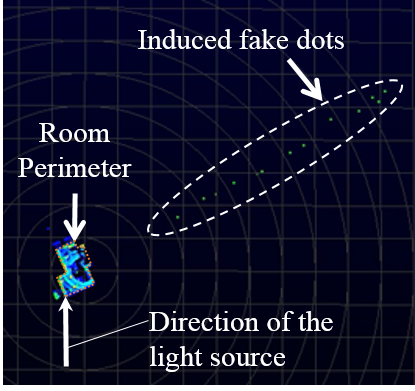
\includegraphics[width=\textwidth]{img/lidar/interference_angle_control.png}
		\caption{Spoofing an obstacle at a different angle of the spoofer}
		\label{fig:shinInterferenceAngle}
	\end{subfigure}
	\quad
	\begin{subfigure}[c]{0.55\textwidth}
		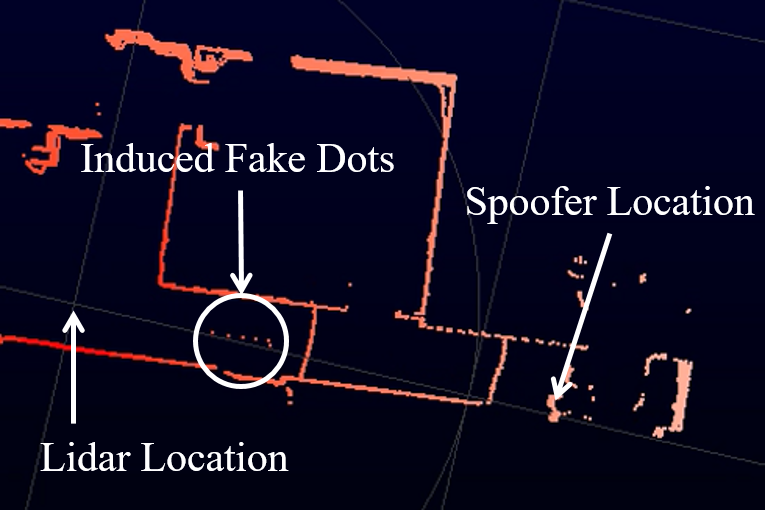
\includegraphics[width=\textwidth]{img/lidar/interference_distance_control.png}
		\caption{Spoofing an obstacle at a closer distance than the spoofer}
		\label{fig:shinInterferenceDistance}
	\end{subfigure}
	\caption{Spoofing examples on a Velodyne VLP-16 \ac{lidar}, extracted from Source~\cite{Shin2017}. Sub-figure~(\ref{fig:shinInterferenceAngle}) shows the spoofed object at a different angle of the spoofer and sub-figure~(\ref{fig:shinInterferenceDistance}) shows the spoofed object at a different distance than the spoofer.}
	\label{fig:shinInterference}
\end{figure}


\subsection{Two-Dimensional Coplanar \ac{lidar} Interference}
Gunzung Kim\etal, in 2015, presents the first results on multiple \ac{lidar} interference on its three papers~\cite{Kim2015a, Kim2015b, Kim2015c}. The three papers are based on a SICK LMS-511, a 2D \ac{lidar}\footnote{A single laser and photodetector are mounted on a rotating device, measuring several azimuthal angles when the motor rotates, but the polar angle is kept fixed, scanning a single line of the environment.}. Kim\etal setups consist of a box with $\SI{5.3}{\meter} \times \SI{4}{\meter}$~\cite{Kim2015a} or $\SI{5.3}{\meter} \times \SI{5.3}{\meter}$~\cite{Kim2015b, Kim2015c}, being the \acp{lidar} positioned inside. The walls are made of a non-glossy wood and the experimental setup is shown on figure~\ref{fig:kim-setups}. His classification of interference is based on the determination of a majorant and minorant for the distance of the wall, with a 10\% tolerance around the mean value.

\begin{figure}[!ht]
	\centering
	\begin{subfigure}[c]{0.45\textwidth}
		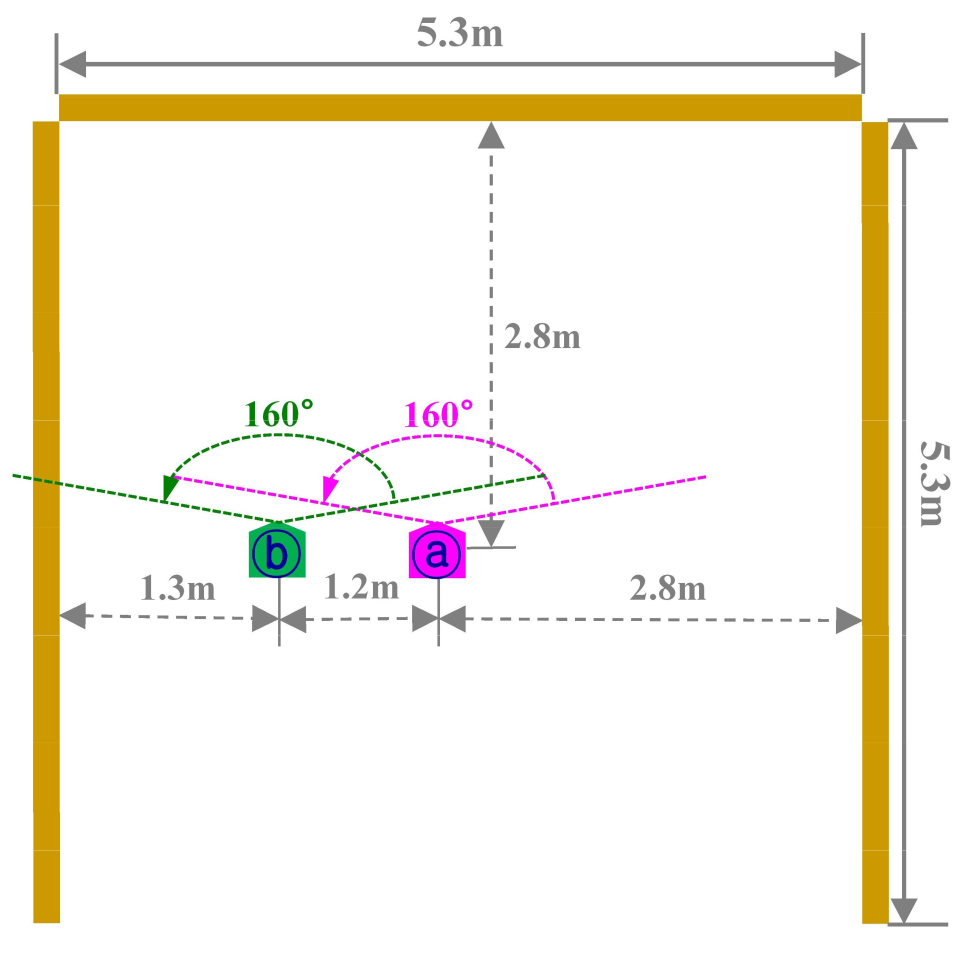
\includegraphics[width=\textwidth]{img/lidar-interference/kim-setup-side-by-side-1.png}
		\caption{\textit{Side-by-Side \#1}.}
		\label{fig:kim-side-by-side-1}
	\end{subfigure}
	\quad
	\begin{subfigure}[c]{0.45\textwidth}
		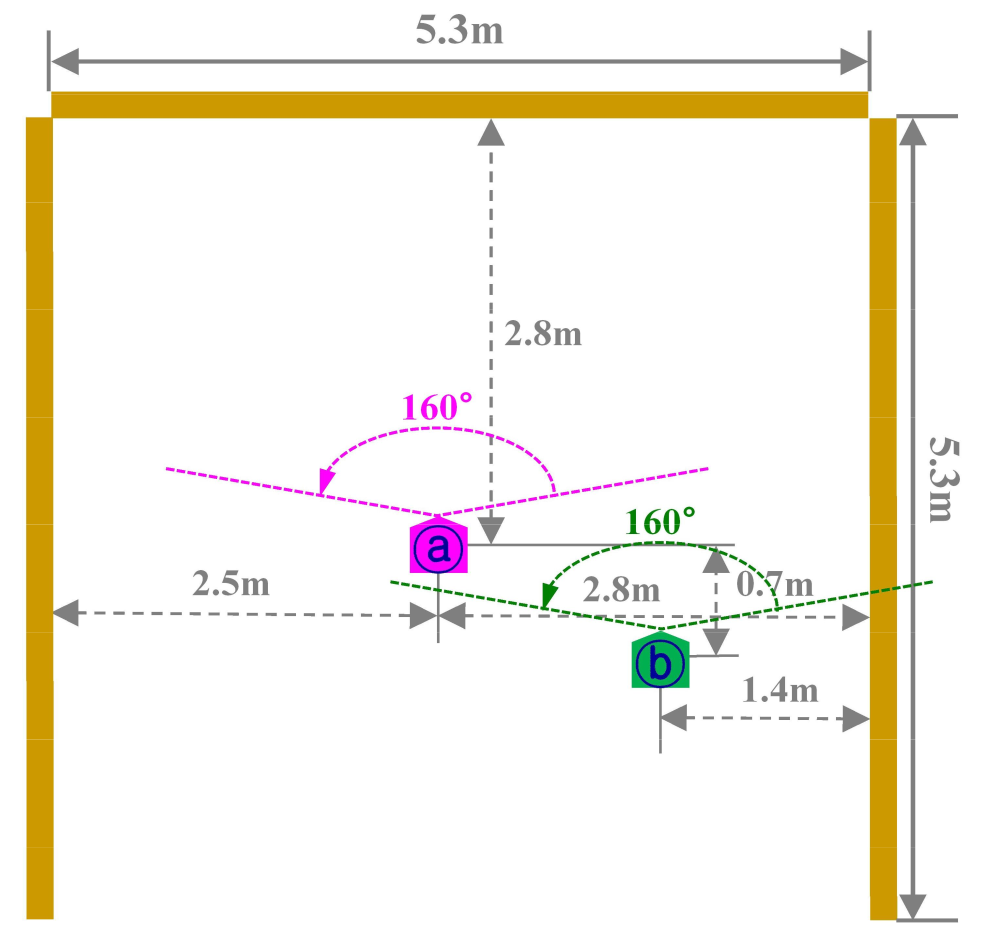
\includegraphics[width=\textwidth]{img/lidar-interference/kim-setup-side-by-side-2.png}
		\caption{\textit{Side-by-Side \#2}.}
		\label{fig:kim-side-by-side-2}
	\end{subfigure}
	\\ \vspace{4mm}
	\centering
	\begin{subfigure}[c]{0.45\textwidth}
		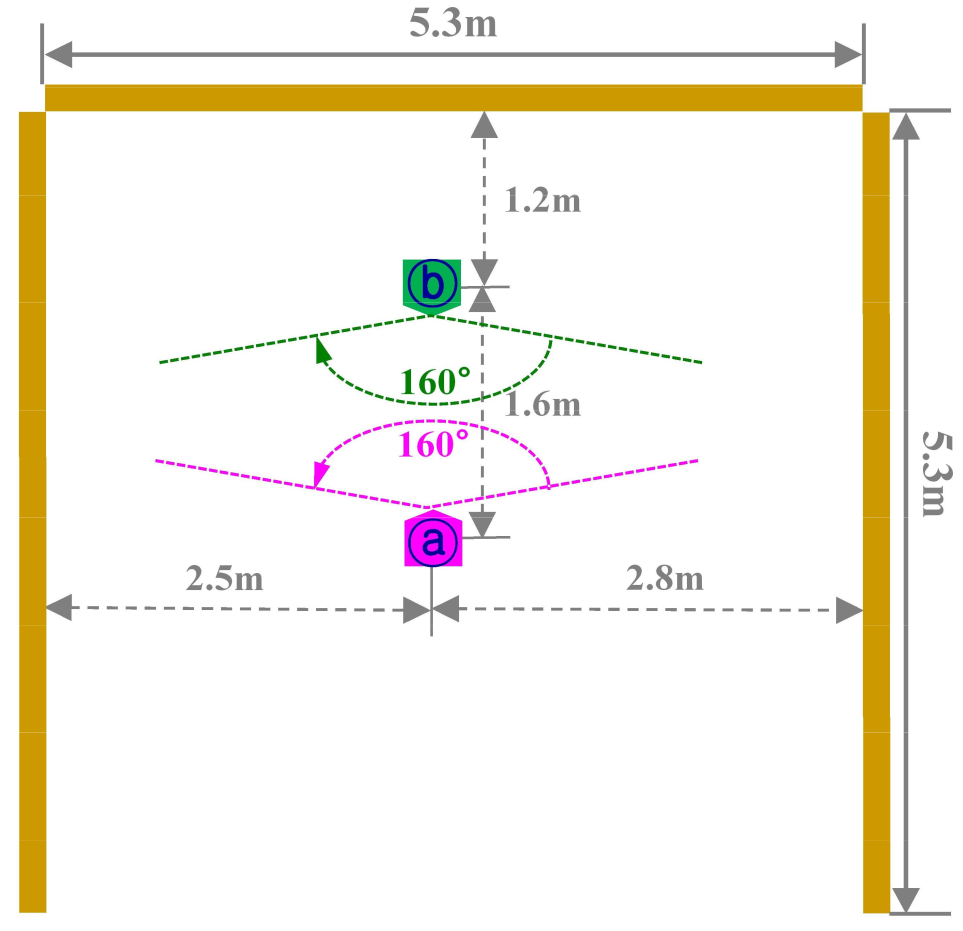
\includegraphics[width=\textwidth]{img/lidar-interference/kim-setup-face-to-face.png}
		\caption{\textit{Face-to-Face}.}
		\label{fig:kim-face-to-face}
	\end{subfigure}
	\quad
	\begin{subfigure}[c]{0.45\textwidth}
		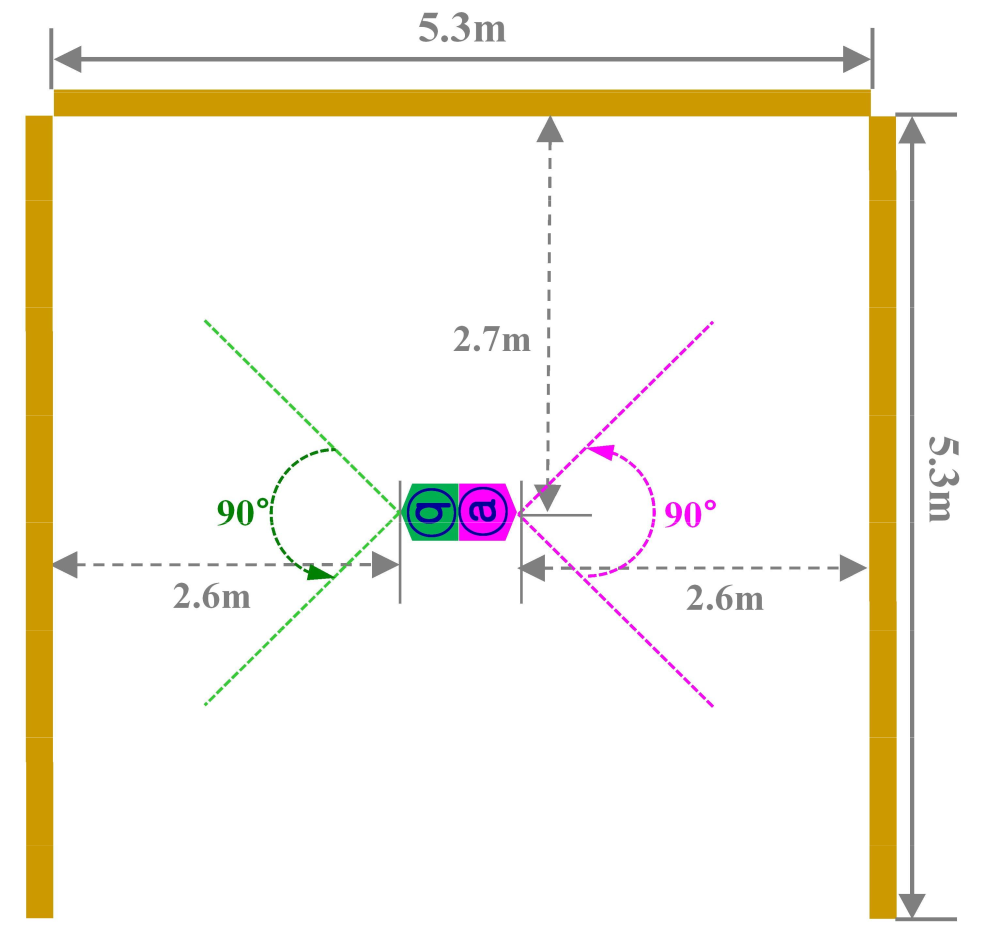
\includegraphics[width=\textwidth]{img/lidar-interference/kim-setup-back-to-back.png}
		\caption{\textit{Back-to-back}.}
		\label{fig:kim-back-to-back}
	\end{subfigure}

	\caption{Experimental setups devised by Gunzung Kim\etal, as detailed on~\cite{Kim2017}. Sub-figure~(\subref{fig:kim-side-by-side-1}) and (\subref{fig:kim-side-by-side-2}) consist of an interference setup where the victim and interferer \ac{lidar} are adjacent to each other. Sub-figure~(\subref{fig:kim-face-to-face}) tests the interference when the two \acp{lidar} are on each other \ac{fov} and sub-figure~(\subref{fig:kim-back-to-back}) when the \acp{lidar} are not on each other \ac{fov}.}
	\label{fig:kim-setups}
\end{figure}


% Kim \etal research despite using a 2D \ac{lidar} instead of a 3D \ac{lidar} is the only study to use two independent 2D \ac{lidar}s interfering with each other. Kim \etal results indicate that interference has spatial and temporal locality \cite{Kim2015} and in any given time, in Kim's setup, a data point has 0.05 \% probability of being interfered \cite{Kim2015}. The former states that if a particular angle is interfered, the following angles are likely to also be interfered; while the latter indicates that if a measure is interfered, on the following frame that same measure is also likely to be interfered. 

Kim\etal tests show the temporal and spatial locality of the data. Temporal locality implies that a given angular direction is more likely to be interfered if it was interfered in the past, indicating that interference persists through time. Spatial locality implies that, for a current scan, if an interference occurs, it is more likely that the next angle will also be interfered, indicating that interference persists through space. 

The experiment conducted in~\cite{Kim2015a} captured a ground-truth model for 4 hours and the interference data for 50 hours. For a given angle position, Kim concluded that for his experimental setup, 4.4\% of the total number of full line scans were interfered, but that number only translate to one in every 2000 point (0.05\% interfered points for the total number of registered points). When considering the nature of interference, spatial interference is rare: 78\% of the interfered points are not interfered on their next measurement (against 15\% that are), and only 7\% of the angular positions are interfered consecutively 3 or more times, for a record of 13 (meaning \SI{0.5}{\second} of interference). For consecutive interference on nearby azimuthal angles on the same scan, only 30\% of the interference happens within single angular step and 26\% on a second. The largest consecutive number of angles with interference are 102, which translates to \SI{25.5}{\degree}.

In~\cite{Kim2015b}, Kim~\etal reports new tests on \ac{lidar} interference, adding two new tests: a side-by-side with a small displacement and a face-to-face test. In~\cite{Kim2015c} a back-to-back test is also performed. Note that despite the experimental setup \textit{Side by side \#1} being identical to the setup on~\cite{Kim2015a}, disagreements on all evaluated metrics occur. Therefore, for this test, the results discussed before, taken from~\cite{Kim2015a}, and results presented on table~\ref{tab:kim_2015_results}, based on~\cite{Kim2015b, Kim2015c}, are not in agreement. No explanations are provided for such difference and the issue is not addressed by Kim\etal on~\cite{Kim2015b, Kim2015c}.

\begin{table}[!ht]
	\centering
	\renewcommand{\arraystretch}{1.3}
	\begin{tabular}{@{}p{3.5cm}C{3cm}C{4cm}@{}}
			\toprule
			Experimental Setup Codename & \% of Lines Interfered & Relative Frequence of Interfered Points \\
			\midrule
			Side-by-side \#1 & $1.795$                & $3.103\E^{-5}$  \\
			Side-by-side \#2 & $10.33$                & $1.667\E^{-4}$ \\ \midrule
			Face-to-Face     & $1.433$                & $2.583\E^{-5}$  \\ \midrule
			Back-to-Back A   & $0.211$                & $3.387\E^{-6}$  \\
			Back-to-Back B   & $0.216$                & $3.514\E^{-6}$  \\ \bottomrule
		\end{tabular}
		\caption{Summary of Kim's\etal the interference results from~\cite{Kim2015b, Kim2015c}, for all tests. In the second column, the percentage of lines with a single interfered point are presented. The third column corresponds to the relative frequency of interfered point for all the points.}
	\label{tab:kim_2015_results}
\end{table}

The results of the second column, \textit{\% of Lines Interfered}, characterizes the number of lines on which interference as been found. For every test scenario on this column, the line interference caused are mostly non-consecutive (above 90\% for Face to Face and 94.3\% for all the other tests).

The third column, \textit{Relative Frequence of Interfered Points}, characterizes the number of points that have been interfered regarding all points taken. The relative frequency of the interference is low, with the relation between the interfered and the total number of points being on the order of magnitude of $10^{-6}$ to $10^{-4}$. Despite the maximum of consecutive spatial interference (4 scans), more than $99.7\%$ of all interferences happen isolated on a given azimuth angle, with no repetition on the next scan for the same interfered angle~\cite{Kim2015c}. 



% To the best of the author's knowledge, despite the relevance of the topic to a society of self-driving cars, there are only three different studies available


In 2017, Kim\etal present the results on the above papers~\cite{Kim2015a, Kim2015b, Kim2015c}, extending its research by performing an intensity analysis~\cite{Kim2017}. His findings are that on a mutual interference scenario, the intensity of the received laser pulses varies significantly, confirming Hebert and Krotkov early findings that on a \ac{lidar} system range and intensity measures are not completely independent and interfering with one affects the results of other~\cite{Hebert}.

In the same paper, he also introduces a theoretical analysis of the multipath interference based on a Lambertian distribution for modelling the reflections on the walls~\cite{Kim2017}. The model lacks generality, as it assumes average values for several parameters and some simplifications on the multipath interference, but allows to conclude that:

\begin{enumerate}
	\item After the second reflection on an obstacle, the attenuation suffered by the light beam is not sufficient for the receiving \ac{lidar} to detect it as an interference;
	\item Direct interference (on Kim's experimental setup and hardware) is likely to saturate the receiver of the interfered \ac{lidar}, which may or may not be considered a valid measurement by the hardware;
	\item Indirect interference with only one reflection can be interpreted as a valid measurement, since the intensity of the received interfered beam is similar to the intensity of a valid measurement beam.
\end{enumerate}

In 2019, Gerald Popko\etal~\cite{Popko2019a} presents a mathematical description on how stationary, coplanar and circular 2D scanning \ac{lidar} can interfere through beam path interference of the optical \ac{fov}. Based on his description, he repeats Kim's\etal experiments (see figure~\ref{fig:kim-setups}), proposing a new statistical interference detector, instead of Kim's maximum distance minorant and majorant~\cite{Kim2015a}, and also performs a Monte-Carlo simulation~\cite{Popko2019b}. Popko\etal findings are that:

\begin{enumerate}
	\item the interference behavior depends majorly on the target geometry and beam intersection, and not on radiometric considerations;
	\item simulating the \ac{lidar} interference is not yet reliable, since for the model developed only the scattered interference provided a value close to the real value measured;
	\item the direct interference is dominant over the scattering interference;
	\item the direct interference is mainly responsible for small distance measurement errors, while scattering interference is mainly present for large distance measurement errors;
\end{enumerate}

Lastly, Popko \etal interference results are two orders of magnitude higher than Kim's \etal measurements, $1.041 \%$~\cite{Popko2019b} vs $0.05\%$~\cite{Kim2015a}.

\subsection{A departing note on \ac{lidar} interference}
On a departing note, \ac{tof} \ac{lidar} is the mainstream \ac{lidar} for autonomous vehicles and the automotive industry, while being the less robust to crosstalk from other \ac{tof} \acp{lidar}. So far, the studies presented on \ac{lidar} interference are scarce and not representative, focused only on two-dimensional \acp{lidar}, i.e., \acp{lidar} that only scan a single line. Answers about the relevance of \ac{lidar} interference are yet to be given and more tests are required, to fully profile the interference and its impacts on autonomous driving. Robust alternatives to crosstalk, both from a technological and signal processing standpoint are also desirable.
